%% LyX 2.3.4.2 created this file.  For more info, see http://www.lyx.org/.
%% Do not edit unless you really know what you are doing.
\documentclass[a4paper,oneside,english]{book}
\usepackage[T1]{fontenc}
\usepackage[latin9]{inputenc}
\setcounter{secnumdepth}{3}
\setcounter{tocdepth}{3}
\synctex=-1
\usepackage{units}
\usepackage{amsmath}
\usepackage{amsthm}
\usepackage{amssymb}
\usepackage{esint}

\makeatletter

%%%%%%%%%%%%%%%%%%%%%%%%%%%%%% LyX specific LaTeX commands.
\pdfpageheight\paperheight
\pdfpagewidth\paperwidth

%% Because html converters don't know tabularnewline
\providecommand{\tabularnewline}{\\}

%%%%%%%%%%%%%%%%%%%%%%%%%%%%%% Textclass specific LaTeX commands.
\numberwithin{equation}{section}
\numberwithin{figure}{section}
\theoremstyle{definition}
\newtheorem*{defn*}{\protect\definitionname}
\theoremstyle{plain}
\newtheorem{thm}{\protect\theoremname}
\theoremstyle{remark}
\newtheorem{rem}[thm]{\protect\remarkname}
\theoremstyle{definition}
\newtheorem{example}[thm]{\protect\examplename}
\theoremstyle{definition}
\newtheorem{defn}[thm]{\protect\definitionname}

%%%%%%%%%%%%%%%%%%%%%%%%%%%%%% User specified LaTeX commands.
\usepackage{mathtools}
\usepackage{tikz}
\usepackage{pgfplots}
\usepackage{tikz-3dplot}
\tdplotsetmaincoords{60}{115}
\pgfplotsset{compat=newest}

\usetikzlibrary{backgrounds}
\usetikzlibrary{arrows}
\usetikzlibrary{shapes,shapes.geometric,shapes.misc}

% this style is applied by default to any tikzpicture included via \tikzfig
\tikzstyle{tikzfig}=[baseline=-0.25em,scale=0.5]

% these are dummy properties used by TikZiT, but ignored by LaTex
\pgfkeys{/tikz/tikzit fill/.initial=0}
\pgfkeys{/tikz/tikzit draw/.initial=0}
\pgfkeys{/tikz/tikzit shape/.initial=0}
\pgfkeys{/tikz/tikzit category/.initial=0}

% standard layers used in .tikz files
\pgfdeclarelayer{edgelayer}
\pgfdeclarelayer{nodelayer}
\pgfsetlayers{background,edgelayer,nodelayer,main}

% style for blank nodes
\tikzstyle{none}=[inner sep=0mm]

\makeatother

\usepackage{babel}
\providecommand{\definitionname}{Definition}
\providecommand{\examplename}{Example}
\providecommand{\remarkname}{Remark}
\providecommand{\theoremname}{Theorem}

\begin{document}
\title{General Relativity Notes}
\author{Li Yuanheng}

\maketitle
\tableofcontents{}

\part{Mathematics}

\chapter{Tensor Calculus}
\begin{enumerate}
\item What is Tensor Calculus?
\begin{defn*}
Study of how tensors change over space
\end{defn*}
\item Why would you want to study it?
\item What do I need to start?
\end{enumerate}

\section{Multi-Variable Calculus}

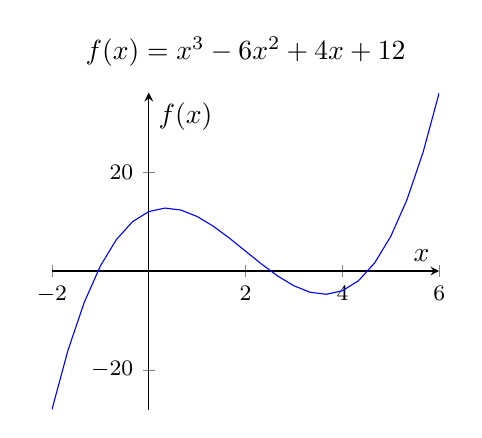
\begin{tikzpicture}
    \begin{axis}[
            title={$f(x)=x^3-6x^2+4x+12$},
            xlabel=$x$,
			ylabel=$f(x)$,
            small,
			axis lines=center
        ]
        \addplot[
            blue,
            domain=-2:6,
        ]
        {x^3-6*x^2+4*x+12};
    \end{axis}
\end{tikzpicture}

slope at $x=f'(x)=\frac{df}{dx}$
\begin{itemize}
\item Power Rule:
\[
\frac{d}{dx}x^{n}=nx^{n-1}
\]
\item Exponential Rule:
\[
\frac{d}{dx}e^{x}=e^{x}
\]
\item Trig Rule:
\begin{align*}
\frac{d}{dx}\sin x & =\cos x\\
\frac{d}{dx}\cos x & =-\sin x
\end{align*}
\item Sum Rule:
\[
\frac{d}{dx}\left(f(x)+g(x)\right)=\frac{df}{dx}+\frac{dg}{dx}
\]
\item Product Rule: 
\[
\frac{d}{dx}(f(x)g(x))=\frac{df}{dx}g(x)+f(x)\frac{df}{dg}
\]
\item Chain Rule:
\[
\frac{d}{dx}(f(g(x)))=\frac{df}{dg}\frac{dg}{dx}
\]
\end{itemize}
\begin{rem}
$\frac{dx}{du}=\frac{du}{dx}$
\end{rem}


\subsection{Derivative(multi-variable)}

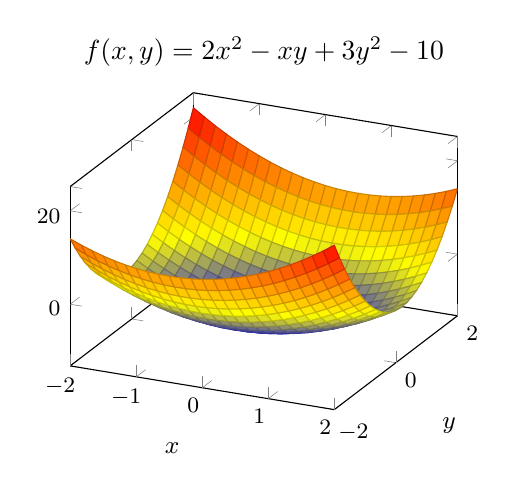
\begin{tikzpicture}
    \begin{axis}[
            title={$f(x,y)=2x^2-xy+3y^2-10$},
            xlabel=$x$, ylabel=$y$,
            small
        ]
        \addplot3[
            surf,
            domain=-2:2,
            domain y=-2:2,
        ]
        {2*x^2-x*y+5*y^2-10};
    \end{axis}
\end{tikzpicture}
\begin{rem}
$\frac{dx}{du}\neq\frac{du}{dx}$
\end{rem}


\subsection{Chain Rule (multi-variable)}

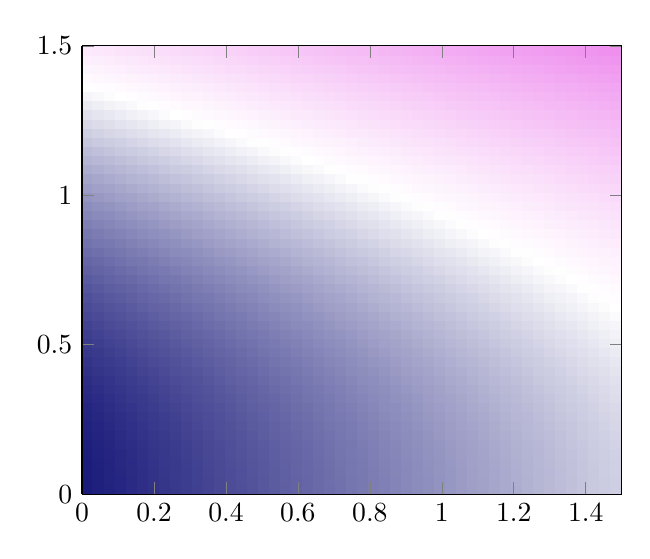
\begin{tikzpicture}
	\begin{axis}[view/h=0,view/v=90,colormap/violet]
	\addplot3[
		surf,
		shader=flat,
		samples=50,
		domain=0:1.5,] 
		{y^2+x-1/2};
	\end{axis}
\end{tikzpicture}

\begin{align*}
\frac{df}{dt} & =\frac{\partial f}{\partial x}\frac{\partial x}{\partial t}+\frac{\partial f}{\partial y}\frac{\partial y}{\partial t}\\
\frac{df}{dt} & =\sum_{i}\frac{\partial f}{\partial q^{i}}\frac{\partial q^{i}}{\partial t}=\frac{\partial f}{\partial q^{i}}\frac{\partial q^{i}}{\partial t}
\end{align*}


\subsection{Gradient of a function}

\[
\nabla=\left[\begin{array}{c}
\frac{\partial}{\partial x}\\
\frac{\partial}{\partial y}
\end{array}\right]
\]
\begin{align*}
df & =\frac{\partial f}{\partial x}dx+\frac{\partial f}{\partial y}dy
\end{align*}

\[
\boxed{df=\sum_{i}\frac{\partial f}{\partial q^{i}}dq^{i}=\frac{\partial f}{\partial q^{i}}dq^{i}}
\]


\subsection{Arc Length}

\begin{align*}
arc\ length & =\int\left\Vert \frac{d\vec{R}}{dt}\right\Vert dt\\
 & =\int\sqrt{\frac{d\vec{R}}{dt}\cdot\frac{d\vec{R}}{dt}}dt\\
 & =\int\sqrt{\left(\frac{\partial\vec{R}}{\partial x}\frac{dx}{dt}+\frac{\partial\vec{R}}{\partial y}\frac{dy}{dt}\right)\cdot\left(\frac{\partial\vec{R}}{\partial x}\frac{dx}{dt}+\frac{\partial\vec{R}}{\partial y}\frac{dy}{dt}\right)}dt\\
 & =\int\sqrt{\left(\frac{dx}{dt}\right)^{2}\left(\frac{\partial\vec{R}}{\partial x}\cdot\frac{\partial\vec{R}}{\partial x}\right)+2\frac{dx}{dt}\frac{dy}{dt}\left(\frac{\partial\vec{R}}{\partial x}\cdot\frac{\partial\vec{R}}{\partial y}\right)+\left(\frac{dy}{dt}\right)^{2}\left(\frac{\partial\vec{R}}{\partial y}\cdot\frac{\partial\vec{R}}{\partial y}\right)}
\end{align*}

\[
\left\Vert \frac{d\vec{R}}{dt}\right\Vert =\sqrt{\sum_{i}\sum_{j}\frac{dq^{i}}{dt}\frac{dq^{j}}{dt}\left(\frac{\partial\vec{R}}{\partial q^{i}}\cdot\frac{\partial\vec{R}}{\partial q^{j}}\right)}=\sqrt{\frac{dq^{i}}{dt}\frac{dq^{j}}{dt}\left(\frac{\partial\vec{R}}{\partial q^{i}}\cdot\frac{\partial\vec{R}}{\partial q^{j}}\right)}
\]


\subsection{Summary}
\begin{itemize}
\item Multi-Variable Chain Rule
\[
\boxed{\frac{df}{dt}=\sum_{i}\frac{\partial T}{\partial q^{i}}\frac{\partial q^{i}}{\partial t}=\frac{\partial T}{\partial q^{i}}\frac{\partial q^{i}}{\partial t}}
\]
\item Total Differential Formula
\[
\boxed{df=\sum_{i}\frac{\partial f}{\partial q^{i}}dq^{i}=\frac{\partial f}{\partial q^{i}}dq^{i}}
\]
\item Velocity Vector tangent to a Curve (magnitude)
\[
\boxed{\left\Vert \frac{d\vec{R}}{dt}\right\Vert =\sqrt{\sum_{i}\sum_{j}\frac{dq^{i}}{dt}\frac{dq^{j}}{dt}\left(\frac{\partial\vec{R}}{\partial q^{i}}\cdot\frac{\partial\vec{R}}{\partial q^{j}}\right)}=\sqrt{\frac{dq^{i}}{dt}\frac{dq^{j}}{dt}\left(\frac{\partial\vec{R}}{\partial q^{i}}\cdot\frac{\partial\vec{R}}{\partial q^{j}}\right)}}
\]
\end{itemize}

\section{Cartesian and Polar Coordinate}

\begin{align*}
\cos\theta & =\frac{x}{r} & x & =r\cos\theta\\
\sin\theta & =\frac{y}{r} & y & =r\sin\theta
\end{align*}

\begin{align*}
\tan\theta & =\frac{y}{x}\\
\theta & =\arctan\left(\frac{y}{x}\right)\\
r & =\sqrt{x^{2}+y^{2}}
\end{align*}

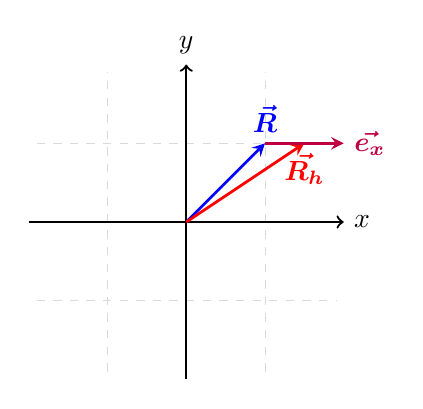
\begin{tikzpicture}
	\draw[help lines, color=gray!30, dashed] (-1.9,-1.9) grid (1.9,1.9);
	\draw[->,thick] (-2,0)--(2,0) node[right]{$x$};
	\draw[->,thick] (0,-2)--(0,2) node[above]{$y$};
	\draw[line width=1pt,blue,-stealth](0,0)--(1,1) node[anchor=south]{$\boldsymbol{\vec{R}}$};
	\draw[line width=1pt,red,-stealth](0,0)--(1.5,1) node[anchor=north]{$\boldsymbol{\vec{R_h}}$};
	\draw[line width=1pt,purple,-stealth](1,1)--(2,1) node[anchor=west]{$\boldsymbol{\vec{e_x}}$};
\end{tikzpicture}    

\begin{align}
\frac{\partial\vec{R}}{\partial x} & =\lim_{h\rightarrow0}\frac{\vec{R_{h}}\left(x+h,y\right)-\vec{R}\left(x,y\right)}{h}\\
 & \equiv\vec{e_{x}}
\end{align}


\section{The Jacobian}

\begin{align*}
\tilde{\vec{e_{1}}} & =2\vec{e_{1}}+1\vec{e_{2}}\\
\tilde{\vec{e_{2}}} & =-\frac{1}{2}\vec{e_{1}}+\frac{1}{4}\vec{e_{2}}
\end{align*}

\[
F=\begin{bmatrix}2 & -\nicefrac{1}{2}\\
1 & \nicefrac{1}{4}
\end{bmatrix}
\]

\begin{alignat*}{3}
\tilde{\vec{e_{r}}}= &  & \vec{e_{x}}+ &  & \vec{e_{y}}\\
\tilde{\vec{e_{\theta}}}= &  & \vec{e_{x}}+ &  & \vec{e_{y}}\\
\frac{\partial\vec{R}}{\partial r}= & \frac{\partial x}{\partial r} & \frac{\partial\vec{R}}{\partial x}+ & \frac{\partial y}{\partial r} & \frac{\partial\vec{R}}{\partial y}\\
\frac{\partial\vec{R}}{\partial\theta}= & \frac{\partial x}{\partial\theta} & \frac{\partial\vec{R}}{\partial x}+ & \frac{\partial y}{\partial\theta} & \frac{\partial\vec{R}}{\partial y}
\end{alignat*}


\section{Derivatives are Vectors}

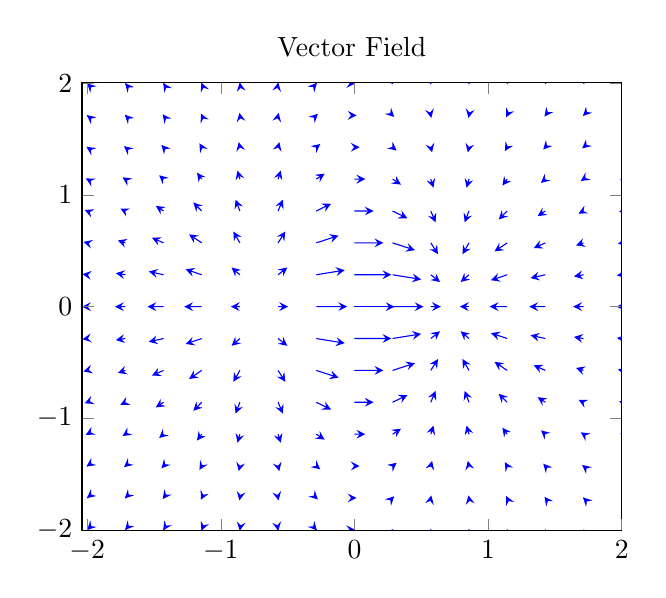
\begin{tikzpicture}
	\begin{axis}[
		title={Vector Field},
		domain=-2:2,
		view={0}{90},
		axis background/.style={fill=white},
	]
		\addplot3 [
			blue,-stealth,samples=15,
			quiver={
				u={exp(0-x^2-y^2)*(1-2*x^2)},
				v={exp(0-x^2-y^2)*(-2*x*y)},
				scale arrows=0.3,
			},
			] {exp(0-x^2-y^2)*x};
	\end{axis}
\end{tikzpicture}

$\vec{R}$ is an position vector. 

Tengent Vector to a Curve parametized by $\lambda$:

\begin{alignat*}{3}
\vec{v} & =v^{1}\vec{e_{1}}+v^{2}\vec{e_{2}} &  & =v^{i}\vec{e_{i}} &  & =\tilde{v^{i}}\tilde{\vec{e_{i}}}\\
\frac{d\vec{R}}{d\lambda} & =\frac{dx}{d\lambda}\frac{\partial\vec{R}}{\partial x}+\frac{dy}{d\lambda}\frac{\partial\vec{R}}{\partial y} &  & =\frac{dc^{i}}{d\lambda}\frac{\partial\vec{R}}{\partial c^{i}} &  & =\frac{dp^{i}}{d\lambda}\frac{\partial\vec{R}}{\partial p^{i}}
\end{alignat*}


\section{Derivative Transformation Rules (Contravariance)}

\begin{alignat*}{2}
\vec{v} & =v^{i}\vec{e_{i}} &  & =\tilde{v^{i}}\tilde{\vec{e_{i}}}\\
\frac{d}{d\lambda} & =\frac{dc^{i}}{d\lambda}\frac{\partial}{\partial c^{i}} &  & =\frac{dp^{i}}{d\lambda}\frac{\partial}{\partial p^{i}}
\end{alignat*}
\begin{align*}
\boxed{\begin{aligned}\tilde{\vec{e_{j}}} & =F_{j}^{i}\vec{e_{i}}\\
\vec{e_{j}} & =B_{j}^{i}\tilde{\vec{e_{i}}}
\end{aligned}
} & \quad\boxed{\begin{aligned}\tilde{v^{i}} & =B_{j}^{i}v^{i}\\
v^{i} & =F_{j}^{i}\tilde{v^{j}}
\end{aligned}
}\\
\boxed{\begin{aligned}\frac{\partial}{\partial p^{j}} & =\frac{\partial c^{i}}{\partial p^{j}}\frac{\partial}{\partial c^{i}}\\
\frac{\partial}{\partial c^{j}} & =\frac{\partial p^{i}}{\partial c^{j}}\frac{\partial}{\partial p^{i}}
\end{aligned}
} & \quad\boxed{\begin{aligned}\frac{dp^{i}}{d\lambda} & =\frac{\partial p^{i}}{\partial c^{j}}\frac{dc^{j}}{d\lambda}\\
\frac{dc^{i}}{d\lambda} & =\frac{\partial c^{i}}{\partial p^{j}}\frac{dp^{j}}{d\lambda}
\end{aligned}
}
\end{align*}

Tangent Vector Space $T$ with point $p$ on surface $M$:

\[
T_{p}M
\]


\section{Differentials are Covectors}

\[
\boxed{df\left(\vec{v}\right)\textnormal{ is proportional to the steepness of }f\textnormal{ in the direction of }\vec{v}}
\]

\[
\boxed{df\left(\vec{v}\right)\textnormal{ is proportional to the length of }\vec{v}}\textnormal{ }
\]

\[
\boxed{df\left(\vec{v}\right)\textnormal{tells us the rate of change of }f\textnormal{ when moving at velocity }\vec{v}.}
\]

\[
\boxed{df\left(\vec{v}\right)\textnormal{is the \emph{directional derivative}}.}
\]

\[
\boxed{df\left(\vec{v}\right)}=\nabla_{\vec{v}}f=D_{\vec{v}}f=\frac{\partial f}{\partial\vec{v}}=\boxed{\nabla f\cdot\vec{v}}
\]


\section{Covector Field Components}

\[
\textnormal{Scalar Field }f\rightarrow_{d}\textnormal{Covector Field }df
\]

\begin{align*}
\frac{d}{d\lambda} & =\frac{dx}{d\lambda}\frac{\partial}{\partial x}+\frac{dy}{d\lambda}\frac{\partial}{\partial y}\\
df & =Adx+Bdy
\end{align*}

Dual basis(basis covector):

\[
\boxed{\epsilon^{i}\left(\vec{e_{j}}\right)=\delta_{j}^{i}}
\]

\[
\boxed{dc^{i}\left(\frac{\partial}{\partial c^{j}}\right)=\left(\frac{\partial c^{i}}{\partial c^{j}}\right)=\delta_{j}^{i}}
\]

\begin{align*}
\frac{df}{d\lambda} & =\frac{\partial f}{\partial x}\frac{dx}{d\lambda}+\frac{\partial f}{\partial y}\frac{dy}{d\lambda}\\
df\left(\frac{d}{d\lambda}\right) & =\frac{\partial f}{\partial x}\frac{dx}{d\lambda}+\frac{\partial f}{\partial y}\frac{dy}{d\lambda}\\
df\left(\frac{d}{d\lambda}\right) & =\frac{\partial f}{\partial x}dx\left(\frac{d}{d\lambda}\right)+\frac{\partial f}{\partial y}dy\left(\frac{d}{d\lambda}\right)\\
df\left(\frac{d}{d\lambda}\right) & =\left(\frac{\partial f}{\partial x}dx+\frac{\partial f}{\partial y}dy\right)\left(\frac{d}{d\lambda}\right)\\
df & =\frac{\partial f}{\partial x}dx+\frac{\partial f}{\partial y}dy
\end{align*}

\[
\boxed{\begin{aligned}\alpha & =\alpha_{i}\epsilon^{i}=\tilde{\alpha_{i}}\tilde{\epsilon^{i}}\\
df & =\frac{\partial f}{\partial c^{i}}dc^{i}=\frac{\partial f}{\partial p^{i}}dp^{i}
\end{aligned}
}
\]


\section{Covector Field Transformation Rules(Covariance)}

Basis Covectors(Contravariant):

\begin{align*}
dp^{i} & =\frac{\partial p^{i}}{\partial c^{j}}dc^{j}\\
dc^{i} & =\frac{\partial c^{i}}{\partial p^{j}}dp^{j}
\end{align*}

Covecotr Components(Covariant):

\begin{align*}
\frac{\partial f}{\partial p^{j}} & =\frac{\partial c^{i}}{\partial p^{j}}\frac{\partial f}{\partial c^{i}}\\
\frac{\partial f}{\partial c^{j}} & =\frac{\partial p^{i}}{\partial c^{j}}\frac{\partial f}{\partial p^{i}}
\end{align*}


\section{The Metric Tensor and Arc Length}

\[
\begin{split}\left\Vert \frac{d\vec{R}}{dt}\right\Vert  & =\sqrt{\sum_{i}\sum_{j}\frac{dq^{i}}{dt}\frac{dq^{j}}{dt}\left(\frac{\partial\vec{R}}{\partial q^{i}}\cdot\frac{\partial\vec{R}}{\partial q^{j}}\right)}\\
 & =\sqrt{\frac{dq^{i}}{dt}\frac{dq^{j}}{dt}\left(\frac{\partial\vec{R}}{\partial q^{i}}\cdot\frac{\partial\vec{R}}{\partial q^{j}}\right)}\\
 & =\sqrt{\frac{dq^{i}}{dt}\frac{dq^{j}}{dt}g_{ij}}
\end{split}
\]


\section{The Metric Tensor in Curved Spaces}

\subsection{Extrinsic Geometry}

Map 2D plane into 3D coordinate

\[
\left(u,v\right)\mapsto\left(X\left(u,v\right),Y\left(u,v\right),Z\left(u,v\right)\right)
\]

\begin{align*}
X & =\cos v\sin u\\
Y & =\sin v\sin u\\
Z & =\cos u
\end{align*}

\begin{example}
$\lambda\mapsto\left(u=\lambda,v=\lambda\right)$

\begin{align*}
X & =\cos\lambda\sin\lambda\\
Y & =\sin\lambda\sin\lambda\\
Z & =\cos\lambda
\end{align*}

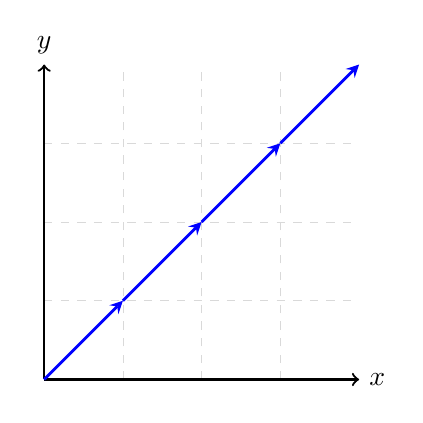
\begin{tikzpicture}
	\draw[help lines, color=gray!30, dashed] (0,0) grid (3.9,3.9);
	\draw[->,thick] (0,0)--(4,0) node[right]{$x$};
	\draw[->,thick] (0,0)--(0,4) node[above]{$y$};
	\draw[line width=1pt,blue,-stealth](0,0)--(1,1);
	\draw[line width=1pt,blue,-stealth](1,1)--(2,2);
	\draw[line width=1pt,blue,-stealth](2,2)--(3,3);
	\draw[line width=1pt,blue,-stealth](3,3)--(4,4);
\end{tikzpicture}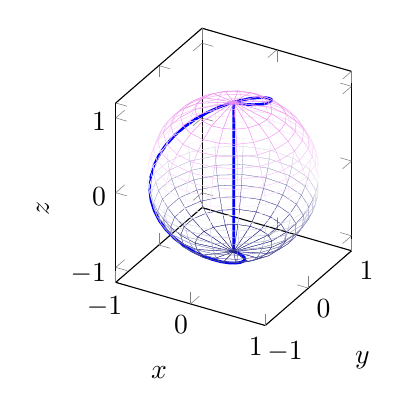
\begin{tikzpicture}[rotate around y=60]
\begin{axis}[view={30}{30},
             xmin=-1, xmax=1, ymin=-1, ymax=1,
             xlabel=$x$, ylabel=$y$, zlabel=$z$,
             unit vector ratio = 1 1 1
            ]
  \addplot3[blue,line width=1pt,variable=\u,domain=0:1,samples=45]( {cos(360*1*u)*sin(180*u))}, {sin(360*1*u)*sin(180*u)}, {cos(180*u)} );
\addplot3[mesh,z buffer=sort,samples=20,variable=\u,domain=-1:1,variable y=\v,y domain=0:2*pi,colormap/violet,line width=0.1pt]({sqrt(1-u^2) * cos(deg(v))},{sqrt( 1-u^2 ) * sin(deg(v))},u);
\end{axis}
\end{tikzpicture}

\[
\textnormal{arc length}=\intop\left\Vert \frac{d\vec{R}}{d\lambda}\right\Vert d\lambda
\]

arc length$\mapsto$basis vector component 

\begin{equation}
\begin{split}\left\Vert \frac{d\vec{R}}{d\lambda}\right\Vert ^{2} & =\frac{d\vec{R}}{d\lambda}\cdot\frac{d\vec{R}}{d\lambda}\\
 & =\left(\frac{dX}{d\lambda}\frac{\partial\vec{R}}{\partial X}+\frac{dY}{d\lambda}\frac{\partial\vec{R}}{\partial Y}+\frac{dZ}{d\lambda}\frac{\partial\vec{R}}{\partial Z}\right)\cdot\left(\frac{dX}{d\lambda}\frac{\partial\vec{R}}{\partial X}+\frac{dY}{d\lambda}\frac{\partial\vec{R}}{\partial Y}+\frac{dZ}{d\lambda}\frac{\partial\vec{R}}{\partial Z}\right)\\
 & =\left(\frac{dX}{d\lambda}\right)^{2}\left(\frac{\partial\vec{R}}{\partial X}\cdot\frac{\partial\vec{R}}{\partial X}\right)+\left(\frac{dY}{d\lambda}\right)^{2}\left(\frac{\partial\vec{R}}{\partial Y}\cdot\frac{\partial\vec{R}}{\partial Y}\right)+\left(\frac{dZ}{d\lambda}\right)^{2}\left(\frac{\partial\vec{R}}{\partial Z}\cdot\frac{\partial\vec{R}}{\partial Z}\right)\\
 & \qquad+2\left(\frac{dX}{d\lambda}\cdot\frac{dY}{d\lambda}\right)\left(\frac{\partial\vec{R}}{\partial X}\cdot\frac{\partial\vec{R}}{\partial Y}\right)+2\left(\frac{dX}{d\lambda}\cdot\frac{dZ}{d\lambda}\right)\left(\frac{\partial\vec{R}}{\partial X}\cdot\frac{\partial\vec{R}}{\partial Z}\right)+2\left(\frac{dY}{d\lambda}\cdot\frac{dZ}{d\lambda}\right)\left(\frac{\partial\vec{R}}{\partial Y}\cdot\frac{\partial\vec{R}}{\partial Z}\right)\\
 & =\left(\frac{dX}{d\lambda}\right)^{2}+\left(\frac{dY}{d\lambda}\right)^{2}+\left(\frac{dZ}{d\lambda}\right)^{2}\\
 & =\begin{bmatrix}\frac{dX}{d\lambda} & \frac{dY}{d\lambda} & \frac{dZ}{d\lambda}\end{bmatrix}\begin{bmatrix}\frac{\partial\vec{R}}{\partial X}\cdot\frac{\partial\vec{R}}{\partial X} & \frac{\partial\vec{R}}{\partial X}\cdot\frac{\partial\vec{R}}{\partial Y} & \frac{\partial\vec{R}}{\partial X}\cdot\frac{\partial\vec{R}}{\partial Z}\\
\frac{\partial\vec{R}}{\partial Y}\cdot\frac{\partial\vec{R}}{\partial X} & \frac{\partial\vec{R}}{\partial Y}\cdot\frac{\partial\vec{R}}{\partial Y} & \frac{\partial\vec{R}}{\partial Y}\cdot\frac{\partial\vec{R}}{\partial Z}\\
\frac{\partial\vec{R}}{\partial Z}\cdot\frac{\partial\vec{R}}{\partial X} & \frac{\partial\vec{R}}{\partial Z}\cdot\frac{\partial\vec{R}}{\partial Y} & \frac{\partial\vec{R}}{\partial Z}\cdot\frac{\partial\vec{R}}{\partial Z}
\end{bmatrix}\begin{bmatrix}\frac{dX}{d\lambda}\\
\frac{dY}{d\lambda}\\
\frac{dZ}{d\lambda}
\end{bmatrix}\\
 & =\begin{bmatrix}\frac{dX}{d\lambda} & \frac{dY}{d\lambda} & \frac{dZ}{d\lambda}\end{bmatrix}\begin{bmatrix}g_{ij}\end{bmatrix}\begin{bmatrix}\frac{dX}{d\lambda}\\
\frac{dY}{d\lambda}\\
\frac{dZ}{d\lambda}
\end{bmatrix}\\
 & =\begin{bmatrix}\frac{dX}{d\lambda} & \frac{dY}{d\lambda} & \frac{dZ}{d\lambda}\end{bmatrix}\begin{bmatrix}1 & 0 & 0\\
0 & 1 & 0\\
0 & 0 & 1
\end{bmatrix}\begin{bmatrix}\frac{dX}{d\lambda}\\
\frac{dY}{d\lambda}\\
\frac{dZ}{d\lambda}
\end{bmatrix}
\end{split}
\end{equation}

\begin{align*}
\frac{dX}{d\lambda} & =\cos\left(2\lambda\right)\\
\frac{dY}{d\lambda} & =\sin\left(2\lambda\right)\\
\frac{dZ}{d\lambda} & =-\sin\left(\lambda\right)
\end{align*}

\begin{align*}
\left\Vert \frac{d\vec{R}}{d\lambda}\right\Vert ^{2} & =\left(\frac{dX}{d\lambda}\right)^{2}+\left(\frac{dY}{d\lambda}\right)^{2}+\left(\frac{dZ}{d\lambda}\right)^{2}\\
 & =1+\left(\sin\left(\lambda\right)\right)^{2}
\end{align*}

\begin{align*}
\textnormal{arc length} & =\int_{0}^{1}\left\Vert \frac{d\vec{R}}{d\lambda}\right\Vert d\lambda\\
 & =\int_{0}^{1}\sqrt{1+\left(\sin\left(\lambda\right)\right)^{2}}d\lambda\\
 & \approx1.12389\neq\sqrt{2}
\end{align*}
\end{example}


\subsection{Intrinsic Geometry}

\begin{align*}
\left\Vert \frac{d\vec{R}}{d\lambda}\right\Vert ^{2} & =\frac{d\vec{R}}{d\lambda}\cdot\frac{d\vec{R}}{d\lambda}\\
 & =\left(\frac{du}{d\lambda}\frac{\partial\vec{R}}{\partial u}+\frac{dv}{d\lambda}\frac{\partial\vec{R}}{\partial v}\right)\cdot\left(\frac{du}{d\lambda}\frac{\partial\vec{R}}{\partial u}+\frac{dv}{d\lambda}\frac{\partial\vec{R}}{\partial v}\right)\\
 & =\left(\frac{du}{d\lambda}\right)^{2}\left(\frac{\partial\vec{R}}{\partial u}\cdot\frac{\partial\vec{R}}{\partial u}\right)+\left(\frac{dv}{d\lambda}\right)^{2}\left(\frac{\partial\vec{R}}{\partial v}\cdot\frac{\partial\vec{R}}{\partial v}\right)+2\left(\frac{du}{d\lambda}\cdot\frac{dv}{d\lambda}\right)\left(\frac{\partial\vec{R}}{\partial u}\cdot\frac{\partial\vec{R}}{\partial v}\right)\\
 & =\begin{bmatrix}\frac{du}{d\lambda} & \frac{dv}{d\lambda}\end{bmatrix}\begin{bmatrix}\frac{\partial\vec{R}}{\partial u}\cdot\frac{\partial\vec{R}}{\partial u} & \frac{\partial\vec{R}}{\partial u}\cdot\frac{\partial\vec{R}}{\partial v}\\
\frac{\partial\vec{R}}{\partial v}\cdot\frac{\partial\vec{R}}{\partial u} & \frac{\partial\vec{R}}{\partial v}\cdot\frac{\partial\vec{R}}{\partial v}
\end{bmatrix}\begin{bmatrix}\frac{du}{d\lambda}\\
\frac{dv}{d\lambda}
\end{bmatrix}\\
 & =\begin{bmatrix}\frac{du}{d\lambda} & \frac{dv}{d\lambda}\end{bmatrix}\begin{bmatrix}\vec{e_{u}}\cdot\vec{e_{u}} & \vec{e_{u}}\cdot\vec{e_{v}}\\
\vec{e_{v}}\cdot\vec{e_{u}} & \vec{e_{v}}\cdot\vec{e_{v}}
\end{bmatrix}\begin{bmatrix}\frac{du}{d\lambda}\\
\frac{dv}{d\lambda}
\end{bmatrix}
\end{align*}

$\frac{\partial\vec{R}}{\partial u}\textnormal{ and \ensuremath{\frac{\partial\vec{R}}{\partial v}} can be obtain by translating coordinate system to cartesian via chain rule}$

\begin{align*}
\frac{\partial\vec{R}}{\partial u} & =\vec{e_{u}}\\
 & =\frac{dX}{du}\frac{\partial\vec{R}}{\partial X}+\frac{dY}{du}\frac{\partial\vec{R}}{\partial Y}+\frac{dZ}{du}\frac{\partial\vec{R}}{\partial Z}\\
 & =\frac{dX}{du}\vec{e_{X}}+\frac{dY}{du}\vec{e_{Y}}+\frac{dZ}{du}\vec{e_{Z}}\\
 & =\cos v\cos u\frac{\partial\vec{R}}{\partial X}+\sin v\cos u\frac{\partial\vec{R}}{\partial Y}-\sin u\frac{\partial\vec{R}}{\partial Z}\\
\frac{\partial\vec{R}}{\partial v} & =\vec{e_{v}}\\
 & =\frac{dX}{dv}\frac{\partial\vec{R}}{\partial X}+\frac{dY}{dv}\frac{\partial\vec{R}}{\partial Y}+\frac{dZ}{dv}\frac{\partial\vec{R}}{\partial Z}\\
 & =-\sin v\sin u\frac{\partial\vec{R}}{\partial X}+\cos v\sin u\frac{\partial\vec{R}}{\partial Y}
\end{align*}

\[
\begin{bmatrix}g_{ij}\end{bmatrix}=\begin{bmatrix}\vec{e_{u}}\cdot\vec{e_{u}} & \vec{e_{u}}\cdot\vec{e_{v}}\\
\vec{e_{v}}\cdot\vec{e_{u}} & \vec{e_{v}}\cdot\vec{e_{v}}
\end{bmatrix}=\begin{bmatrix}1 & 0\\
0 & \left(\sin\left(u\right)\right)^{2}
\end{bmatrix}
\]

\begin{align*}
\left\Vert \frac{d\vec{R}}{d\lambda}\right\Vert ^{2} & =\begin{bmatrix}\frac{du}{d\lambda} & \frac{dv}{d\lambda}\end{bmatrix}\begin{bmatrix}\vec{e_{u}}\cdot\vec{e_{u}} & \vec{e_{u}}\cdot\vec{e_{v}}\\
\vec{e_{v}}\cdot\vec{e_{u}} & \vec{e_{v}}\cdot\vec{e_{v}}
\end{bmatrix}\begin{bmatrix}\frac{du}{d\lambda}\\
\frac{dv}{d\lambda}
\end{bmatrix}\\
 & =\begin{bmatrix}\frac{du}{d\lambda} & \frac{dv}{d\lambda}\end{bmatrix}\begin{bmatrix}1 & 0\\
0 & \left(\sin\left(u\right)\right)^{2}
\end{bmatrix}\begin{bmatrix}\frac{du}{d\lambda}\\
\frac{dv}{d\lambda}
\end{bmatrix}\\
 & =\left(\frac{du}{d\lambda}\right)^{2}+\left(\sin\left(u\right)\right)^{2}\left(\frac{dv}{d\lambda}\right)^{2}
\end{align*}

with example above:

\[
\frac{du}{d\lambda}=\frac{dv}{d\lambda}=1
\]

\[
\left\Vert \frac{d\vec{R}}{d\lambda}\right\Vert ^{2}=1+\left(\sin\left(u\right)\right)^{2}
\]

\begin{align*}
\textnormal{arc length} & =\int_{0}^{1}\left\Vert \frac{d\vec{R}}{d\lambda}\right\Vert d\lambda\\
 & =\int_{0}^{1}\sqrt{1+\left(\sin\left(\lambda\right)\right)^{2}}d\lambda\\
 & \approx1.12389\neq\sqrt{2}
\end{align*}


\subsection{Metric Tensor Field Execises}

\subsubsection{Cylinder}

\subsubsection{Saddle Surface}

\section{Gradient vs $d$ operator}
\begin{description}
\item [{$\nabla f$}] ``Del'' $f$\\
aka ``Gradient'' of $f$\\
Vector Field
\item [{$df$}] ``dee'' $f$\\
aka ``Differential'' of $f$\\
aka ``Exterior Derivative'' of $f$
\end{description}
\begin{tabular}{|c|c|}
\hline 
$\nabla f$ & $df$\tabularnewline
\hline 
\hline 
``Del'' $f$ & ``dee'' $f$\tabularnewline
\hline 
``Gradient'' of $f$ & ``Differential'' of $f$\tabularnewline
\hline 
 & ``Exterior Derivative'' of $f$\tabularnewline
\hline 
\multicolumn{2}{|c|}{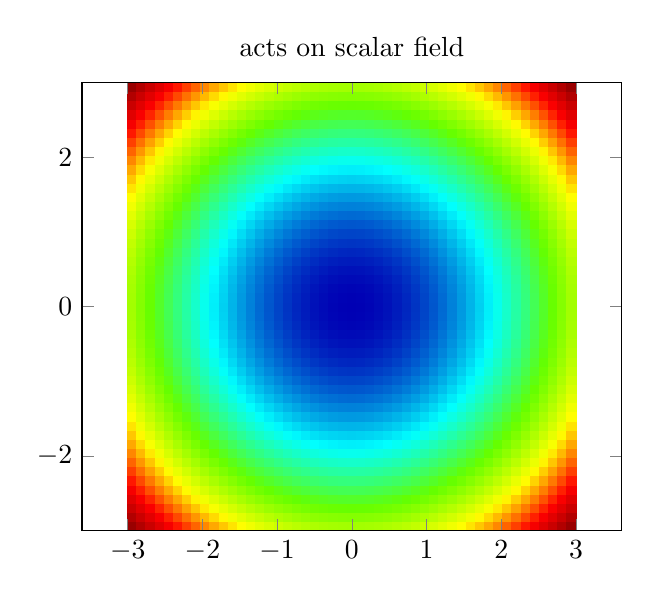
\begin{tikzpicture}
	\begin{axis}[title={acts on scalar field},view/h=0,view/v=90,colormap/bluered,unit vector ratio=1 1 1]
	\addplot3[
		surf,
		shader=flat,
		samples=50,
		domain=-3:3,] 
		{y^2+x^2};
	\end{axis}
\end{tikzpicture}}\tabularnewline
\hline 
Vector Field & Covector Field(1-form)\tabularnewline
\hline 
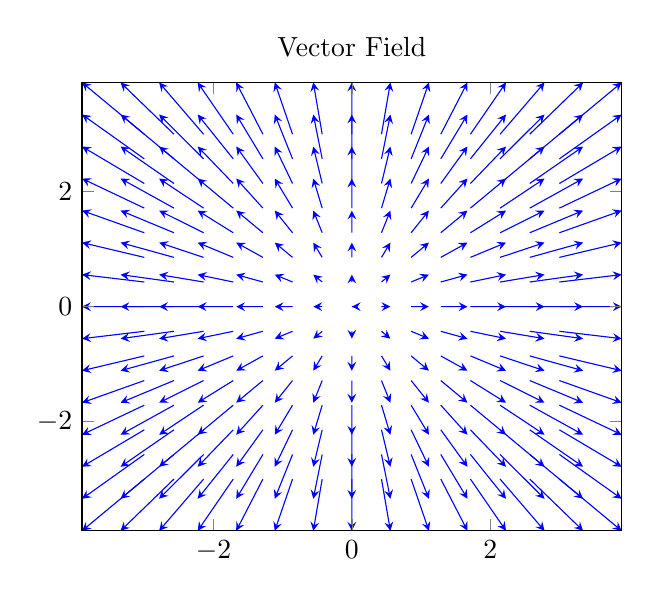
\begin{tikzpicture}
	\begin{axis}[
		title={Vector Field},
		domain=-3:3,
		view={0}{90},
		axis background/.style={fill=white},
	]
		\addplot3 [
			blue,-stealth,samples=15,
			quiver={
				u={x},
				v={y},
				scale arrows=0.3,
			},
			] {x^2+y^2};
	\end{axis}
\end{tikzpicture} & \tabularnewline
\hline 
\end{tabular} 

Convert components $df$ and $\nabla f$:

\begin{align*}
\left(\nabla f\right)^{i}g_{ij} & =\frac{\partial f}{\partial c^{j}}\\
\left(\nabla f\right)^{k} & =\mathfrak{g}^{jk}\frac{\partial f}{\partial c^{j}}
\end{align*}
\begin{align*}
\flat\left(\nabla f\right) & =df\\
\sharp\left(df\right) & =\nabla f
\end{align*}
\[
\boxed{df=\nabla f\cdot\underline{\quad}=g_{ij}\left(\nabla f\right)^{i}dc^{j}}
\]


\section{Geodesics and Christoffel Symbols}
\begin{defn}
In curved space, a straight path has zero tangential acceleration
when travel along it at constant speed.
\end{defn}

\begin{rem}
Geodesic curves are curves where the acceleration vector is normal
to the surface.
\end{rem}

\[
\frac{d^{2}\vec{R}}{d\lambda^{2}}=\left(\frac{d^{2}\vec{R}}{d\lambda^{2}}\right)^{\textnormal{normal}}+\underbrace{\left(\frac{d^{2}\vec{R}}{d\lambda^{2}}\right)^{\textnormal{tangential}}}_{=0}
\]

\[
\textnormal{Velocity Vector (always in tangent plane)}=\frac{d\vec{R}}{d\lambda}=\frac{du}{d\lambda}\frac{\partial\vec{R}}{\partial u}+\frac{dv}{d\lambda}\frac{\partial\vec{R}}{\partial v}
\]
\begin{align*}
\textnormal{Acceleration Vector:}\\
\frac{d}{d\lambda}\left(\frac{\partial\vec{R}}{\partial\lambda}\right) & =\frac{d}{d\lambda}\left(\frac{du}{d\lambda}\frac{\partial\vec{R}}{\partial u}+\frac{dv}{d\lambda}\frac{\partial\vec{R}}{\partial v}\right)\\
 & =\frac{d}{d\lambda}\left(\frac{du}{d\lambda}\frac{\partial\vec{R}}{\partial u}\right)+\frac{d}{d\lambda}\left(\frac{dv}{d\lambda}\frac{\partial\vec{R}}{\partial v}\right)\\
 & =\frac{d^{2}u}{d\lambda^{2}}\frac{\partial\vec{R}}{\partial u}+\frac{du}{d\lambda}\underbrace{\left(\frac{d}{d\lambda}\frac{\partial\vec{R}}{\partial u}\right)}_{\boxed{\begin{aligned} & =\left(\frac{du}{d\lambda}\frac{\partial}{\partial u}+\frac{dv}{d\lambda}\frac{\partial}{\partial v}\right)\frac{\partial\vec{R}}{\partial u}\\
 & =\frac{du}{d\lambda}\frac{\partial^{2}\vec{R}}{\partial u^{2}}+\frac{dv}{d\lambda}\frac{\partial^{2}\vec{R}}{\partial u\partial v}
\end{aligned}
}}+\frac{d^{2}v}{d\lambda^{2}}\frac{\partial\vec{R}}{\partial v}+\frac{dv}{d\lambda}\left(\frac{d}{d\lambda}\frac{\partial\vec{R}}{\partial v}\right)\\
 & =\frac{d^{2}u}{d\lambda^{2}}\frac{\partial\vec{R}}{\partial u}+\frac{du}{d\lambda}\left(\frac{du}{d\lambda}\frac{\partial^{2}\vec{R}}{\partial u^{2}}+\frac{dv}{d\lambda}\frac{\partial^{2}\vec{R}}{\partial u\partial v}\right)\\
 & \qquad+\frac{d^{2}v}{d\lambda^{2}}\frac{\partial\vec{R}}{\partial v}+\frac{dv}{d\lambda}\left(\frac{du}{d\lambda}\frac{\partial^{2}\vec{R}}{\partial v\partial u}+\frac{dv}{d\lambda}\frac{\partial^{2}\vec{R}}{\partial v^{2}}\right)\\
 & =\underbrace{\frac{d^{2}u}{d\lambda^{2}}\frac{\partial\vec{R}}{\partial u}+\frac{d^{2}v}{d\lambda^{2}}\frac{\partial\vec{R}}{\partial v}}_{\textnormal{tangential}}\\
 & \qquad+\left(\frac{du}{d\lambda}\right)^{2}\frac{\partial^{2}\vec{R}}{\partial u^{2}}+\frac{du}{d\lambda}\frac{dv}{d\lambda}\frac{\partial^{2}\vec{R}}{\partial u\partial v}+\frac{dv}{d\lambda}\frac{du}{d\lambda}\frac{\partial^{2}\vec{R}}{\partial v\partial u}+\left(\frac{dv}{d\lambda}\right)^{2}\frac{\partial^{2}\vec{R}}{\partial v^{2}}\\
\textnormal{} & =\underbrace{\frac{d^{2}u^{i}}{d\lambda^{2}}\frac{\partial\vec{R}}{\partial u^{i}}}_{\textnormal{tangential}}+\frac{du^{i}}{d\lambda}\frac{du^{j}}{d\lambda}\frac{\partial^{2}\vec{R}}{\partial u^{i}\partial u^{j}}
\end{align*}

Denote $\frac{\partial^{2}\vec{R}}{\partial u^{i}\partial u^{j}}$
in 3D using tangential basis vector $\frac{\partial\vec{R}}{\partial u^{1}}$,
$\frac{\partial\vec{R}}{\partial u^{2}}$ and normal basis vector
$\hat{n}$:

\[
\boxed{\textnormal{Second Fundamental Form }L_{ij}\textnormal{ is the normal components of \ensuremath{\frac{\partial^{2}\vec{R}}{\partial u^{i}\partial u^{j}}}}}
\]
\[
\boxed{\textnormal{Christoffel Symbol }\Gamma_{ij}^{k}\textnormal{ is the tangential components of \ensuremath{\frac{\partial^{2}\vec{R}}{\partial u^{i}\partial u^{j}}}}}
\]

\begin{equation}
\begin{split}\frac{\partial^{2}\vec{R}}{\partial u^{i}\partial u^{j}} & =\Gamma_{ij}^{1}\frac{\partial\vec{R}}{\partial u^{1}}+\Gamma_{ij}^{2}\frac{\partial\vec{R}}{\partial u^{2}}+L_{ij}\hat{n}\\
 & =\Gamma_{ij}^{k}\frac{\partial\vec{R}}{\partial u^{k}}+L_{ij}\hat{n}
\end{split}
\label{eq:}
\end{equation}

\begin{align*}
\frac{\partial^{2}\vec{R}}{\partial u^{i}\partial u^{j}}\cdot\frac{\vec{R}}{\partial u^{l}} & =\left(\Gamma_{ij}^{k}\frac{\partial\vec{R}}{\partial u^{k}}+L_{ij}\hat{n}\right)\cdot\frac{\partial\vec{R}}{\partial u^{l}}\\
 & =\Gamma_{ij}^{k}\frac{\partial\vec{R}}{\partial u^{k}}\cdot\frac{\partial\vec{R}}{\partial u^{l}}+\underbrace{L_{ij}\hat{n}\cdot\frac{\vec{R}}{\partial u^{l}}}_{\textnormal{perpendicular}}\\
 & =\Gamma_{ij}^{k}\frac{\partial\vec{R}}{\partial u^{k}}\cdot\frac{\partial\vec{R}}{\partial u^{l}}\\
 & =\Gamma_{ij}^{k}g_{kl}\\
\frac{\partial^{2}\vec{R}}{\partial u^{i}\partial u^{j}}\cdot\frac{\vec{R}}{\partial u^{l}}\mathfrak{g}^{lm} & =\Gamma_{ij}^{k}g_{kl}\mathfrak{g}^{lm}\\
 & =\Gamma_{ij}^{k}\delta_{k}^{m}\\
 & =\Gamma_{ij}^{m}
\end{align*}

\[
\boxed{\Gamma_{ij}^{m}=\frac{\partial^{2}\vec{R}}{\partial u^{i}\partial u^{j}}\cdot\frac{\vec{R}}{\partial u^{l}}\mathfrak{g}^{lm}}
\]
\begin{align*}
\frac{\partial^{2}\vec{R}}{\partial u^{i}\partial u^{j}}\cdot\hat{n} & =\left(\Gamma_{ij}^{k}\frac{\partial\vec{R}}{\partial u^{k}}+L_{ij}\hat{n}\right)\cdot\hat{n}\\
 & =L_{ij}\left(\hat{n}\cdot\hat{n}\right)\\
\frac{\partial^{2}\vec{R}}{\partial u^{i}\partial u^{j}}\cdot\frac{\vec{e_{i}}\times\vec{e_{j}}}{\left\Vert \vec{e_{i}}\times\vec{e_{j}}\right\Vert } & =L_{ij}\\
\frac{\partial^{2}\vec{R}}{\partial u^{i}\partial u^{j}}\cdot\frac{\frac{\partial\vec{R}}{\partial u^{i}}\times\frac{\partial\vec{R}}{\partial u^{j}}}{\left\Vert \frac{\partial\vec{R}}{\partial u^{i}}\times\frac{\partial\vec{R}}{\partial u^{j}}\right\Vert } & =L_{ij}
\end{align*}

\[
\boxed{L_{ij}=\frac{\partial^{2}\vec{R}}{\partial u^{i}\partial u^{j}}\cdot\frac{\vec{e_{i}}\times\vec{e_{j}}}{\left\Vert \vec{e_{i}}\times\vec{e_{j}}\right\Vert }=\frac{\partial^{2}\vec{R}}{\partial u^{i}\partial u^{j}}\cdot\frac{\frac{\partial\vec{R}}{\partial u^{i}}\times\frac{\partial\vec{R}}{\partial u^{j}}}{\left\Vert \frac{\partial\vec{R}}{\partial u^{i}}\times\frac{\partial\vec{R}}{\partial u^{j}}\right\Vert }}
\]

\begin{align*}
\frac{d}{d\lambda}\left(\frac{\partial\vec{R}}{\partial\lambda}\right) & =\underbrace{\frac{d^{2}u^{i}}{d\lambda^{2}}\frac{\partial\vec{R}}{\partial u^{i}}}_{\textnormal{tangential}}+\frac{du^{i}}{d\lambda}\frac{du^{j}}{d\lambda}\frac{\partial^{2}\vec{R}}{\partial u^{i}\partial u^{j}}\\
 & =\frac{d^{2}u^{i}}{d\lambda^{2}}\frac{\partial\vec{R}}{\partial u^{i}}+\frac{du^{i}}{d\lambda}\frac{du^{j}}{d\lambda}\left(\Gamma_{ij}^{k}\frac{\partial\vec{R}}{\partial u^{k}}+L_{ij}\hat{n}\right)\ref{eq:}\\
 & =\underbrace{\left(\frac{d^{2}u^{k}}{d\lambda^{2}}+\Gamma_{ij}^{k}\frac{du^{i}}{d\lambda}\frac{du^{j}}{d\lambda}\right)}_{\textnormal{tantential component}}\frac{\partial\vec{R}}{\partial u^{k}}+\underbrace{L_{ij}\frac{du^{i}}{d\lambda}\frac{du^{j}}{d\lambda}}_{\textnormal{normal component}}\hat{n}
\end{align*}

for geodesic curve, set tangential component to 0.

\[
\boxed{\textnormal{Geodesic Equation: }\frac{d^{2}u^{k}}{d\lambda^{2}}+\Gamma_{ij}^{k}\frac{du^{i}}{d\lambda}\frac{du^{j}}{d\lambda}=0}
\]

\begin{example}
Geodesic on Flat Plane
\begin{enumerate}
\item Normal position vector on flat plane
\[
\vec{R}\left(u,v\right)=\vec{p}+u\vec{a}+v\vec{b}
\]
\item Calculate partial derivative of variables
\begin{align*}
\frac{\partial\vec{R}}{\partial u} & =\vec{a}\\
\frac{\partial\vec{R}}{\partial v} & =\vec{b}
\end{align*}
\item Calculate second order derivative of variable $u$ and $v$.
\[
\frac{\partial^{2}\vec{R}}{\partial u^{2}}=\frac{\partial^{2}\vec{R}}{\partial v^{2}}=\frac{\partial^{2}\vec{R}}{\partial u\partial v}=\frac{\partial^{2}\vec{R}}{\partial v\partial u}=0
\]
\item Calculate Christoffel Symbol $\Gamma_{ij}^{k}$.
\[
\Gamma_{ij}^{k}=\underbrace{\frac{\partial^{2}\vec{R}}{\partial u^{i}\partial u^{j}}}_{\textnormal{all are 0}}\cdot\frac{\vec{R}}{\partial u^{l}}\mathfrak{g}^{lk}=0
\]
Christoffel Symbol track basis vector changes from point to point,
hence the zero in flat plane.
\item Solve geodesic equation.
\begin{align*}
\frac{d^{2}u^{k}}{d\lambda^{2}}+\Gamma_{ij}^{k}\frac{du^{i}}{d\lambda}\frac{du^{j}}{d\lambda} & =0\\
\frac{d^{2}u^{k}}{d\lambda^{2}} & =0
\end{align*}
Expand,
\[
\textnormal{Solve}\left\{ \begin{array}{cc}
\frac{d^{2}u}{d\lambda^{2}} & =0\\
\frac{d^{2}v}{d\lambda^{2}} & =0
\end{array}\right.
\]
\begin{align*}
\int\int0d\lambda d\lambda & =c_{1}\lambda+c_{2}\\
u & =k_{u}\lambda+u_{0}\\
v & =k_{v}\lambda+v_{0}
\end{align*}
\item Plug in function for $u$ and $v$, solve geodesic equation,
\begin{align*}
\vec{R}\left(u,v\right) & =\vec{p}+u\vec{a}+v\vec{b}\\
 & =\vec{p}+\left(k_{u}\lambda+u_{0}\right)\vec{a}+\left(k_{v}\lambda+v_{0}\right)\vec{b}\\
 & =\vec{p}+k_{u}\lambda\vec{a}+u_{0}\vec{a}+k_{v}\lambda\vec{b}+v_{0}\vec{b}\\
 & =\underbrace{\left(\vec{p}+u_{0}\vec{a}+v_{0}\vec{b}\right)}_{\textnormal{initial position}}+\underbrace{\lambda}_{\textnormal{time}}\underbrace{\left(k_{u}\vec{a}+k_{v}\vec{b}\right)}_{\textnormal{initial velocity}}
\end{align*}
\end{enumerate}
\end{example}

\begin{example}
Geodesic on Sphere
\begin{enumerate}
\item Calculate partial derivative of variables
\begin{align*}
\frac{\partial\vec{R}}{\partial u} & =\frac{dX}{du}\frac{\partial\vec{R}}{\partial X}+\frac{dY}{du}\frac{\partial\vec{R}}{\partial Y}+\frac{dZ}{du}\frac{\partial\vec{R}}{\partial Z}\\
 & =\frac{dX}{du}\vec{e_{X}}+\frac{dY}{du}\vec{e_{Y}}+\frac{dZ}{du}\vec{e_{Z}}\\
 & =\cos v\cos u\frac{\partial\vec{R}}{\partial X}+\sin v\cos u\frac{\partial\vec{R}}{\partial Y}-\sin u\frac{\partial\vec{R}}{\partial Z}\\
\frac{\partial\vec{R}}{\partial v} & =\frac{dX}{dv}\frac{\partial\vec{R}}{\partial X}+\frac{dY}{dv}\frac{\partial\vec{R}}{\partial Y}+\frac{dZ}{dv}\frac{\partial\vec{R}}{\partial Z}\\
 & =-\sin v\sin u\frac{\partial\vec{R}}{\partial X}+\cos v\sin u\frac{\partial\vec{R}}{\partial Y}
\end{align*}
\item Calculate metric tensor
\[
\begin{bmatrix}g_{ij}\end{bmatrix}=\begin{bmatrix}\frac{\partial\vec{R}}{\partial u}\cdot\frac{\partial\vec{R}}{\partial u} & \frac{\partial\vec{R}}{\partial u}\cdot\frac{\partial\vec{R}}{\partial v}\\
\frac{\partial\vec{R}}{\partial v}\cdot\frac{\partial\vec{R}}{\partial u} & \frac{\partial\vec{R}}{\partial v}\cdot\frac{\partial\vec{R}}{\partial v}
\end{bmatrix}=\begin{bmatrix}1 & 0\\
0 & \left(\sin\left(u\right)\right)^{2}
\end{bmatrix}
\]
\item Calculate second order derivative along $u$ and $v$.
\begin{align*}
\frac{\partial^{2}\vec{R}}{\partial u^{2}} & =\frac{\partial}{\partial u}\frac{\partial\vec{R}}{\partial u}=-\cos v\sin u\frac{\partial\vec{R}}{\partial X}-\sin v\sin u\frac{\partial\vec{R}}{\partial Y}-\cos u\frac{\partial\vec{R}}{\partial Z}\\
\frac{\partial^{2}\vec{R}}{\partial v^{2}} & =\frac{\partial}{\partial v}\frac{\partial\vec{R}}{\partial v}=-\cos v\sin u\frac{\partial\vec{R}}{\partial X}-\sin v\sin u\frac{\partial\vec{R}}{\partial Y}\\
\frac{\partial}{\partial v}\left(\frac{\partial\vec{R}}{\partial u}\right) & =\frac{\partial}{\partial u}\left(\frac{\partial\vec{R}}{\partial v}\right)=-\sin v\cos u\frac{\partial\vec{R}}{\partial X}+\cos v\cos u\frac{\partial\vec{R}}{\partial Y}
\end{align*}
\item Calculate Christoffel Symbol $\Gamma_{ij}^{k}$.
\[
\begin{bmatrix}\mathfrak{g^{ij}}\end{bmatrix}=\begin{bmatrix}1 & 0\\
0 & \nicefrac{1}{\left(\sin\left(u\right)\right)^{2}}
\end{bmatrix}
\]
\begin{align*}
\frac{\partial\vec{R}}{\partial u}\frac{\partial^{2}\vec{R}}{\partial u^{2}}=\frac{\partial\vec{R}}{\partial v}\frac{\partial^{2}\vec{R}}{\partial u^{2}} & =0\\
\frac{\partial\vec{R}}{\partial u}\frac{\partial^{2}\vec{R}}{\partial v^{2}} & =-\cos u\sin u\\
\frac{\partial\vec{R}}{\partial u}\frac{\partial^{2}\vec{R}}{\partial v\partial u}=\frac{\partial\vec{R}}{\partial u}\frac{\partial^{2}\vec{R}}{\partial u\partial v} & =0\\
\frac{\partial\vec{R}}{\partial v}\frac{\partial^{2}\vec{R}}{\partial v^{2}} & =0\\
\frac{\partial\vec{R}}{\partial v}\frac{\partial^{2}\vec{R}}{\partial v\partial u}=\frac{\partial\vec{R}}{\partial v}\frac{\partial^{2}\vec{R}}{\partial u\partial v} & =\cos u\sin u
\end{align*}
\[
\Gamma_{ij}^{k}=\frac{\partial^{2}\vec{R}}{\partial u^{i}\partial u^{j}}\cdot\frac{\vec{R}}{\partial u^{l}}\mathfrak{g}^{lk}
\]
\begin{align*}
\Gamma_{ij}^{1} & =\frac{\partial^{2}\vec{R}}{\partial u^{i}\partial u^{j}}\cdot\frac{\vec{R}}{\partial u^{l}}\mathfrak{g}^{l1}\\
 & =\frac{\partial^{2}\vec{R}}{\partial u^{i}\partial u^{j}}\cdot\frac{\vec{R}}{\partial u^{1}}\mathfrak{g}^{11}+\frac{\partial^{2}\vec{R}}{\partial u^{i}\partial u^{j}}\cdot\frac{\vec{R}}{\partial u^{2}}\mathfrak{g}^{21}\\
 & =\frac{\partial^{2}\vec{R}}{\partial u^{i}\partial u^{j}}\cdot\frac{\vec{R}}{\partial u^{1}}\mathfrak{g}^{11}\\
 & =\frac{\partial^{2}\vec{R}}{\partial u^{i}\partial u^{j}}\cdot\frac{\vec{R}}{\partial u^{1}}\\
\Gamma_{ij}^{2} & =\frac{\partial^{2}\vec{R}}{\partial u^{i}\partial u^{j}}\cdot\frac{\vec{R}}{\partial u^{l}}\mathfrak{g}^{l2}\\
 & =\frac{\partial^{2}\vec{R}}{\partial u^{i}\partial u^{j}}\cdot\frac{\vec{R}}{\partial u^{1}}\mathfrak{g}^{12}+\frac{\partial^{2}\vec{R}}{\partial u^{i}\partial u^{j}}\cdot\frac{\vec{R}}{\partial u^{2}}\mathfrak{g}^{22}\\
 & =\frac{\partial^{2}\vec{R}}{\partial u^{i}\partial u^{j}}\cdot\frac{\vec{R}}{\partial u^{2}}\mathfrak{g}^{22}\\
 & =\frac{\partial^{2}\vec{R}}{\partial u^{i}\partial u^{j}}\cdot\frac{\vec{R}}{\partial u^{2}}\left(\frac{1}{\left(\sin\left(u\right)\right)^{2}}\right)
\end{align*}
\begin{align*}
\frac{\partial\vec{R}}{\partial u}\frac{\partial^{2}\vec{R}}{\partial v^{2}} & =\frac{\partial\vec{R}}{\partial u^{1}}\frac{\partial^{2}\vec{R}}{\partial u\partial u}=-\cos u\sin u\\
\frac{\partial\vec{R}}{\partial v}\frac{\partial^{2}\vec{R}}{\partial v\partial u}=\frac{\partial\vec{R}}{\partial u^{2}}\frac{\partial^{2}\vec{R}}{\partial u^{1}\partial u^{2}} & =\cos u\sin u
\end{align*}
\begin{align*}
\Gamma_{22}^{1} & =\frac{\partial^{2}\vec{R}}{\partial u^{2}\partial u^{2}}\cdot\frac{\vec{R}}{\partial u^{1}}=-\cos u\sin u\\
\Gamma_{12}^{2}=\Gamma_{21}^{2} & =\frac{\partial^{2}\vec{R}}{\partial u^{1}\partial u^{2}}\cdot\frac{\vec{R}}{\partial u^{2}}\left(\frac{1}{\left(\sin\left(u\right)\right)^{2}}\right)=\frac{\cos u\sin u}{\left(\sin\left(u\right)\right)^{2}}=\frac{\cos u}{\sin u}
\end{align*}
\begin{align*}
\begin{bmatrix}\Gamma_{ij}^{1}\end{bmatrix} & =\begin{bmatrix}0 & 0\\
0 & -\cos u\sin u
\end{bmatrix}\\
\begin{bmatrix}\Gamma_{ij}^{2}\end{bmatrix} & =\begin{bmatrix}0 & \nicefrac{\cos u}{\sin u}\\
\nicefrac{\cos u}{\sin u} & 0
\end{bmatrix}
\end{align*}
\item Solve geodesic equation.
\begin{align*}
\frac{d^{2}u^{k}}{d\lambda^{2}}+\Gamma_{ij}^{k}\frac{du^{i}}{d\lambda}\frac{du^{j}}{d\lambda} & =0
\end{align*}
Expand,
\[
\textnormal{Solve}\left\{ \begin{array}{cc}
\frac{d^{2}u^{1}}{d\lambda^{2}}+\Gamma_{22}^{1}\frac{du^{i}}{d\lambda}\frac{du^{j}}{d\lambda} & =0\\
\frac{d^{2}u^{2}}{d\lambda^{2}}+\Gamma_{12}^{2}\frac{du^{1}}{d\lambda}\frac{du^{2}}{d\lambda}+\Gamma_{21}^{2}\frac{du^{2}}{d\lambda}\frac{du^{1}}{d\lambda} & =0
\end{array}\right.
\]
Plug in Christoffel Symbols,
\begin{align*}
\frac{d^{2}u^{1}}{d\lambda^{2}}-\cos u\sin u\frac{du^{i}}{d\lambda}\frac{du^{j}}{d\lambda} & =0\\
\frac{d^{2}u^{2}}{d\lambda^{2}}+2\frac{\cos u}{\sin u}\frac{du^{1}}{d\lambda}\frac{du^{2}}{d\lambda} & =0
\end{align*}
\end{enumerate}
\end{example}


\section{Covariant Derivative}
\begin{defn}
Covariant Derivative is a tool to understand the rate of change of
vector (tensor) fields that takes changing basis vectors into account.
\end{defn}


\subsection{Flat Space Definition}

\begin{align}
\vec{v} & =v^{x}\vec{e_{x}}+v^{y}\vec{e_{y}}=v^{i}\vec{e_{i}}\\
\vec{v} & =v^{x}\frac{\partial\vec{R}}{\partial x}+v^{y}\frac{\partial\vec{R}}{\partial y}=v^{i}\frac{\partial\vec{R}}{\partial c^{i}}\\
\vec{v} & =\tilde{v^{r}}\tilde{\vec{e_{r}}}+\tilde{v^{\theta}}\tilde{\vec{e_{\theta}}}=\tilde{v^{i}}\tilde{\vec{e_{i}}}\\
\vec{v} & =\tilde{v^{r}}\frac{\partial\vec{R}}{\partial r}+\tilde{v^{\theta}}\frac{\partial\vec{R}}{\partial r}=\tilde{v^{i}}\frac{\partial\vec{R}}{\partial p^{i}}
\end{align}

\begin{example}
Cartesian Vector Field $\vec{v}=2\vec{e_{x}}+1\vec{e_{y}}$
\begin{equation}
\begin{split}\frac{\partial}{\partial x}\left(\vec{v}\right) & =\frac{\partial}{\partial x}\left(v^{x}\vec{e_{x}}+v^{y}\vec{e_{y}}\right)\\
 & =\frac{\partial}{\partial x}\left(v^{x}\vec{e_{x}}\right)+\frac{\partial}{\partial x}\left(v^{y}\vec{e_{y}}\right)\\
 & =\frac{\partial v^{x}}{\partial x}\vec{e_{x}}+v^{x}\underbrace{\frac{\partial}{\partial x}\left(\vec{e_{x}}\right)}_{\textnormal{0}}+\frac{\partial v^{y}}{\partial x}\vec{e_{y}}+v^{y}\underbrace{\frac{\partial}{\partial x}\left(\vec{e_{y}}\right)}_{\textnormal{0}}\\
 & =\frac{\partial\overbrace{v^{x}}^{\mathbb{\textnormal{const}}}}{\partial x}\vec{e_{x}}+\frac{\partial v^{y}}{\partial x}\vec{e_{y}}\\
 & =\vec{0}
\end{split}
\end{equation}
\end{example}

\begin{example}
Polar Vector Field $\vec{v}=2\tilde{\vec{e_{r}}}+1\tilde{\vec{e_{\theta}}}$

\begin{equation}
\begin{split}\frac{\partial}{\partial\theta}\left(\vec{v}\right) & =\frac{\partial}{\partial\theta}\left(\tilde{v^{r}}\tilde{\vec{e_{r}}}+\tilde{v^{\theta}}\tilde{\vec{e_{\theta}}}\right)\\
 & =\frac{\partial}{\partial\theta}\left(\tilde{v^{r}}\tilde{\vec{e_{r}}}\right)+\frac{\partial}{\partial\theta}\left(\tilde{v^{\theta}}\tilde{\vec{e_{\theta}}}\right)\\
 & =\frac{\partial\tilde{v^{r}}}{\partial\theta}\tilde{\vec{e_{r}}}+\tilde{v^{r}}\frac{\partial}{\partial\theta}\left(\tilde{\vec{e_{r}}}\right)+\frac{\partial\tilde{v^{\theta}}}{\partial\theta}\tilde{\vec{e_{\theta}}}+\tilde{v^{\theta}}\frac{\partial}{\partial\theta}\left(\tilde{\vec{e_{\theta}}}\right)\\
 & =\underbrace{\frac{\partial\tilde{v^{r}}}{\partial\theta}\tilde{\vec{e_{r}}}+\frac{\partial\tilde{v^{\theta}}}{\partial\theta}\tilde{\vec{e_{\theta}}}}_{\textnormal{change of components}}+\underbrace{\tilde{v^{r}}\frac{\partial}{\partial\theta}\left(\tilde{\vec{e_{r}}}\right)+\tilde{v^{\theta}}\frac{\partial}{\partial\theta}\left(\tilde{\vec{e_{\theta}}}\right)}_{\textnormal{change of basis vector}}
\end{split}
\end{equation}

Need to figure out change of basis vector,
\begin{align}
\frac{\partial}{\partial\theta}\left(\vec{v}\right) & =\frac{\partial\tilde{v^{r}}}{\partial\theta}\tilde{\vec{e_{r}}}+\frac{\partial\tilde{v^{\theta}}}{\partial\theta}\tilde{\vec{e_{\theta}}}+\tilde{v^{r}}\frac{\partial}{\partial\theta}\left(\tilde{\vec{e_{r}}}\right)+\tilde{v^{\theta}}\frac{\partial}{\partial\theta}\left(\tilde{\vec{e_{\theta}}}\right)\\
\frac{\partial}{\partial r}\left(\vec{v}\right) & =\frac{\partial\tilde{v^{r}}}{\partial r}\tilde{\vec{e_{r}}}+\frac{\partial\tilde{v^{\theta}}}{\partial r}\tilde{\vec{e_{\theta}}}+\tilde{v^{r}}\frac{\partial}{\partial r}\left(\tilde{\vec{e_{r}}}\right)+\tilde{v^{\theta}}\frac{\partial}{\partial r}\left(\tilde{\vec{e_{\theta}}}\right)
\end{align}

convert to cartesian coordinates,
\begin{equation}
\begin{split}\tilde{\vec{e_{r}}} & =\frac{\partial x}{\partial r}\vec{e_{x}}+\frac{\partial x}{\partial r}\vec{e_{y}}\\
 & =\cos\theta\vec{e_{x}}+\sin\theta\vec{e_{y}}
\end{split}
\end{equation}

\begin{equation}
\begin{split}\tilde{\vec{e_{\theta}}} & =\frac{\partial x}{\partial\theta}\vec{e_{x}}+\frac{\partial x}{\partial\theta}\vec{e_{y}}\\
 & =-r\sin\theta\vec{e_{x}}+r\cos\theta\vec{e_{y}}
\end{split}
\end{equation}

\begin{equation}
\begin{split}\frac{\partial}{\partial\theta}\left(\tilde{\vec{e_{r}}}\right) & =\frac{\partial}{\partial\theta}\left(\cos\theta\vec{e_{x}}+\sin\theta\vec{e_{y}}\right)\\
 & =\frac{\partial}{\partial\theta}\left(\cos\theta\vec{e_{x}}\right)+\frac{\partial}{\partial\theta}\left(\sin\theta\vec{e_{y}}\right)\\
 & =\frac{\partial\cos\theta}{\partial\theta}\vec{e_{x}}+\cos\theta\frac{\partial\overbrace{\vec{e_{x}}}^{\textnormal{const everywhere}}}{\partial\theta}+\frac{\partial\sin\theta}{\partial\theta}\vec{e_{y}}+\sin\theta\frac{\partial\vec{e_{y}}}{\partial\theta}\\
 & =-\sin\theta\vec{e_{x}}+\cos\theta\vec{e_{y}}\\
 & =\frac{\partial}{\partial\theta}\left(\tilde{\vec{e_{r}}}\right)=\frac{\partial}{\partial\theta}\frac{\partial\vec{R}}{\partial r}=\frac{\partial}{\partial r}\frac{\partial\vec{R}}{\partial\theta}=\frac{\partial}{\partial r}\left(\tilde{\vec{e_{\theta}}}\right)
\end{split}
\end{equation}
\begin{equation}
\begin{split}\frac{\partial}{\partial r}\left(\tilde{\vec{e_{r}}}\right) & =\frac{\partial}{\partial r}\left(\cos\theta\vec{e_{x}}+\sin\theta\vec{e_{y}}\right)\\
 & =\frac{\partial}{\partial r}\left(\cos\theta\vec{e_{x}}\right)+\frac{\partial}{\partial r}\left(\sin\theta\vec{e_{y}}\right)\\
 & =\frac{\partial\cos\theta}{\partial r}\vec{e_{x}}+\cos\theta\frac{\partial\overbrace{\vec{e_{x}}}^{\textnormal{const everywhere}}}{\partial r}+\frac{\partial\sin\theta}{\partial r}\vec{e_{y}}+\sin\theta\frac{\partial\vec{e_{y}}}{\partial r}\\
 & =\vec{0}
\end{split}
\end{equation}
\begin{equation}
\begin{split}\frac{\partial}{\partial\theta}\left(\tilde{\vec{e_{\theta}}}\right) & =-r\cos\theta\vec{e_{x}}-\sin\theta\vec{e_{y}}\end{split}
\end{equation}
\begin{equation}
\begin{split}\vec{e_{x}} & =\frac{\partial r}{\partial x}\tilde{\vec{e_{r}}}+\frac{\partial\theta}{\partial x}\tilde{\vec{e_{\theta}}}\\
 & =\left(\frac{x}{\sqrt{x^{2}+y^{2}}}\right)\tilde{\vec{e_{r}}}+\left(-\frac{y}{x^{2}+y^{2}}\right)\tilde{\vec{e_{\theta}}}\\
 & =\left(\frac{x}{r}\right)\tilde{\vec{e_{r}}}+\left(-\frac{y}{r^{2}}\right)\tilde{\vec{e_{\theta}}}\\
 & =\left(\frac{r\cos\theta}{r}\right)\tilde{\vec{e_{r}}}+\left(-\frac{r\sin\theta}{r^{2}}\right)\tilde{\vec{e_{\theta}}}\\
 & =\left(\cos\theta\right)\tilde{\vec{e_{r}}}+\left(-\frac{\sin\theta}{r}\right)\tilde{\vec{e_{\theta}}}
\end{split}
\end{equation}
\begin{equation}
\begin{split}\vec{e_{y}} & =\frac{\partial r}{\partial y}\tilde{\vec{e_{r}}}+\frac{\partial\theta}{\partial y}\tilde{\vec{e_{\theta}}}\\
 & =\left(\frac{y}{\sqrt{x^{2}+y^{2}}}\right)\tilde{\vec{e_{r}}}+\left(\frac{x}{x^{2}+y^{2}}\right)\tilde{\vec{e_{\theta}}}\\
 & =\left(\frac{y}{r}\right)\tilde{\vec{e_{r}}}+\left(\frac{x}{r^{2}}\right)\tilde{\vec{e_{\theta}}}\\
 & =\left(\sin\theta\right)\tilde{\vec{e_{r}}}+\left(\frac{\cos\theta}{r}\right)\tilde{\vec{e_{\theta}}}
\end{split}
\end{equation}

Plug in,

\begin{align}
\frac{\partial}{\partial r}\left(\tilde{\vec{e_{r}}}\right) & =0
\end{align}
\begin{equation}
\begin{split}\frac{\partial}{\partial\theta}\left(\tilde{\vec{e_{r}}}\right)=\frac{\partial}{\partial r}\left(\tilde{\vec{e_{\theta}}}\right) & =-\sin\theta\vec{e_{x}}+\cos\theta\vec{e_{y}}\\
 & =-\sin\theta\left(\left(\cos\theta\right)\tilde{\vec{e_{r}}}+\left(-\frac{\sin\theta}{r}\right)\tilde{\vec{e_{\theta}}}\right)\\
 & \qquad+\cos\theta\left(\left(\sin\theta\right)\tilde{\vec{e_{r}}}+\left(\frac{\cos\theta}{r}\right)\tilde{\vec{e_{\theta}}}\right)\\
 & =\frac{1}{r}\tilde{\vec{e_{\theta}}}
\end{split}
\end{equation}
\begin{equation}
\begin{split}\frac{\partial}{\partial\theta}\left(\tilde{\vec{e_{\theta}}}\right) & =-r\cos\theta\vec{e_{x}}-\sin\theta\vec{e_{y}}\\
 & =-r\cos\theta\left(\left(\cos\theta\right)\tilde{\vec{e_{r}}}+\left(-\frac{\sin\theta}{r}\right)\tilde{\vec{e_{\theta}}}\right)\\
 & \qquad-\sin\theta\left(\left(\sin\theta\right)\tilde{\vec{e_{r}}}+\left(\frac{\cos\theta}{r}\right)\tilde{\vec{e_{\theta}}}\right)\\
 & =-r\tilde{\vec{e_{r}}}
\end{split}
\end{equation}

Plug in,

\begin{equation}
\begin{split}\frac{\partial}{\partial\theta}\left(\vec{v}\right) & =\frac{\partial\tilde{v^{r}}}{\partial\theta}\tilde{\vec{e_{r}}}+\frac{\partial\tilde{v^{\theta}}}{\partial\theta}\tilde{\vec{e_{\theta}}}+\tilde{v^{r}}\frac{\partial}{\partial\theta}\left(\tilde{\vec{e_{r}}}\right)+\tilde{v^{\theta}}\frac{\partial}{\partial\theta}\left(\tilde{\vec{e_{\theta}}}\right)\\
 & =\frac{\partial\tilde{v^{r}}}{\partial\theta}\tilde{\vec{e_{r}}}+\frac{\partial\tilde{v^{\theta}}}{\partial\theta}\tilde{\vec{e_{\theta}}}+\tilde{v^{r}}\left(\frac{1}{r}\tilde{\vec{e_{\theta}}}\right)+\tilde{v^{\theta}}\left(-r\tilde{\vec{e_{r}}}\right)\\
 & =\frac{1}{r}\tilde{\vec{e_{\theta}}}
\end{split}
\end{equation}
\begin{equation}
\begin{split}\frac{\partial}{\partial r}\left(\vec{v}\right) & =\frac{\partial\tilde{v^{r}}}{\partial r}\tilde{\vec{e_{r}}}+\frac{\partial\tilde{v^{\theta}}}{\partial r}\tilde{\vec{e_{\theta}}}+\tilde{v^{r}}\frac{\partial}{\partial r}\left(\tilde{\vec{e_{r}}}\right)+\tilde{v^{\theta}}\frac{\partial}{\partial r}\left(\tilde{\vec{e_{\theta}}}\right)\\
 & =\frac{\partial\tilde{v^{r}}}{\partial r}\tilde{\vec{e_{r}}}+\frac{\partial\tilde{v^{\theta}}}{\partial r}\tilde{\vec{e_{\theta}}}+\tilde{v^{r}}\left(0\right)+\tilde{v^{\theta}}\left(\frac{1}{r}\tilde{\vec{e_{\theta}}}\right)\\
 & =-r\tilde{\vec{e_{r}}}+\frac{2}{r}\tilde{\vec{e_{\theta}}}
\end{split}
\end{equation}

\[
\boxed{\textnormal{Constant Components }\neq\textnormal{ Constant Vector Field}}
\]
\end{example}

\begin{equation}
\boxed{\frac{\partial\vec{e_{j}}}{\partial c^{i}}=\Gamma_{ij}^{1}\vec{e_{1}}+\Gamma_{ij}^{2}\vec{e_{2}}=\Gamma_{ij}^{k}\vec{e_{k}}}
\end{equation}

\begin{equation}
\begin{split}\frac{\partial}{\partial c^{i}}\left(\vec{v}\right) & =\frac{\partial}{\partial c^{i}}\left(v^{j}\vec{e_{j}}\right)\\
 & =\underbrace{\frac{\partial v^{j}}{\partial c^{i}}\vec{e_{j}}}_{\textnormal{components}}+\underbrace{v^{j}\frac{\partial\vec{e_{j}}}{\partial c^{i}}}_{\textnormal{basis vectors}}\\
 & =\frac{\partial v^{j}}{\partial c^{i}}\vec{e_{j}}+v^{j}\Gamma_{ij}^{k}\vec{e_{k}}\\
 & =\frac{\partial v^{k}}{\partial c^{i}}\vec{e_{k}}+v^{j}\Gamma_{ij}^{k}\vec{e_{k}}\\
 & =\left(\frac{\partial v^{k}}{\partial c^{i}}+v^{j}\Gamma_{ij}^{k}\right)\vec{e_{k}}
\end{split}
\end{equation}
\begin{equation}
\textnormal{Flat Space \& Cartesian Coord: }\Gamma_{ij}^{k}=0
\end{equation}
\begin{equation}
\begin{split}\frac{\partial}{\partial p^{i}}\left(\vec{v}\right) & =\frac{\partial}{\partial p^{i}}\left(\tilde{v^{j}}\tilde{\vec{e_{j}}}\right)\\
 & =\underbrace{\frac{\partial\tilde{v^{j}}}{\partial p^{i}}\vec{e_{j}}}_{\textnormal{components}}+\underbrace{\tilde{v^{j}}\frac{\partial\tilde{\vec{e_{j}}}}{\partial p^{i}}}_{\textnormal{basis vectors}}\\
 & =\frac{\partial\tilde{v^{j}}}{\partial p^{i}}\vec{e_{j}}+\tilde{v^{j}}\Gamma_{ij}^{k}\vec{e_{k}}\\
 & =\frac{\partial\tilde{v^{k}}}{\partial p^{i}}\vec{e_{k}}+\tilde{v^{j}}\Gamma_{ij}^{k}\vec{e_{k}}\\
 & =\left(\frac{\partial\tilde{v^{k}}}{\partial p^{i}}+\tilde{v^{j}}\Gamma_{ij}^{k}\right)\vec{e_{k}}
\end{split}
\end{equation}
\begin{align}
\frac{\partial}{\partial r}\left(\tilde{\vec{e_{r}}}\right) & =\Gamma_{rr}^{1}\vec{e_{1}}+\Gamma_{rr}^{2}\vec{e_{2}}=\Gamma_{rr}^{k}\vec{e_{k}}=0\\
\Gamma_{rr}^{k} & =0\\
\Gamma_{rr}^{r} & =0\\
\Gamma_{rr}^{\theta} & =0\\
\frac{\partial}{\partial\theta}\left(\tilde{\vec{e_{\theta}}}\right) & =\Gamma_{\theta\theta}^{r}\vec{e_{r}}+\Gamma_{\theta\theta}^{\theta}\vec{e_{\theta}}=\Gamma_{\theta\theta}^{k}\vec{e_{k}}=-r\tilde{\vec{e_{r}}}\\
\Gamma_{\theta\theta}^{r} & =-r\\
\Gamma_{\theta\theta}^{\theta} & =0
\end{align}
 

\subsection{Extrinsic}
\begin{defn}
Coveriant Derivative $\nabla_{\vec{w}}\vec{v}$

the rate of change of vector field $\vec{v}$ in a direction $\vec{w}$
with the normal component subtracted.
\end{defn}

\begin{equation}
\boxed{\Gamma_{ij}^{k}=\left(\frac{\partial\vec{e_{j}}}{\partial u^{i}}\cdot\vec{e_{l}}\right)\mathfrak{g}^{lk}}
\end{equation}


\subsection{Intrinsic}

Levi-Civita Connection:

\begin{equation}
\boxed{\Gamma_{jk}^{m}=\frac{1}{2}\mathfrak{g}^{im}\left(\frac{\partial g_{ij}}{\partial u^{k}}+\frac{\partial g_{ki}}{\partial u^{j}}-\frac{\partial g_{jk}}{\partial u^{i}}\right)}
\end{equation}

Parallel Transport:

\[
\nabla_{\partial_{i}}T=0
\]


\subsection{Abstract}

\begin{align}
\nabla_{\vec{e_{i}}}\vec{e_{j}} & =\Gamma_{ij}^{k}\vec{e_{k}}\\
\nabla_{\partial_{i}}\left(a\right) & =\frac{\partial a}{\partial u^{i}}\\
\nabla_{\partial_{i}}\left(\vec{v}\right) & =\left(\frac{\partial v^{k}}{\partial u^{i}}+v^{j}\Gamma_{ij}^{k}\right)\vec{e_{k}}\\
\nabla_{\partial_{i}}\left(a\right) & =\left(\frac{\partial a_{k}}{\partial u^{i}}-a_{j}\Gamma_{ik}^{j}\right)\epsilon^{k}\\
\nabla_{\partial_{i}}\left(g\right) & =\left(\frac{\partial g_{rs}}{\partial u^{i}}-g_{ks}\Gamma_{ir}^{k}-g_{rk}\Gamma_{is}^{k}\right)\left(\epsilon^{r}\otimes\epsilon^{s}\right)
\end{align}

\begin{equation}
\boxed{\nabla_{\vec{w}}\left(T\otimes S\right)=\left(\nabla_{\vec{w}}T\right)\otimes S+T\otimes\left(\nabla_{\vec{w}}S\right)}
\end{equation}


\chapter{Spacetime}

\section{Spherical Coordinates}

\begin{align*}
x & =r\sin\theta\cos\phi\\
y & =r\sin\theta\sin\phi\\
z & =r\cos\theta
\end{align*}

\[
\begin{split}\frac{\partial}{\partial r} & =\vec{e_{r}}\\
 & =\frac{\partial x}{\partial r}\frac{\partial}{\partial x}+\frac{\partial y}{\partial r}\frac{\partial}{\partial y}+\frac{\partial z}{\partial r}\frac{\partial}{\partial z}\\
 & =\sin\theta\cos\phi\vec{e_{x}}+\sin\theta\sin\phi\vec{e_{y}}+\cos\theta\vec{e_{z}}
\end{split}
\]

\[
\begin{split}\frac{\partial}{\partial\theta} & =\vec{e_{\theta}}\\
 & =\frac{\partial x}{\partial\theta}\frac{\partial}{\partial x}+\frac{\partial y}{\partial\theta}\frac{\partial}{\partial y}+\frac{\partial z}{\partial\theta}\frac{\partial}{\partial z}\\
 & =r\cos\theta\cos\phi\vec{e_{x}}-r\cos\theta\sin\phi\vec{e_{y}}-r\sin\theta\vec{e_{z}}
\end{split}
\]

\[
\begin{split}\frac{\partial}{\partial\phi} & =\vec{e_{\phi}}\\
 & =\frac{\partial x}{\partial\phi}\frac{\partial}{\partial x}+\frac{\partial y}{\partial\phi}\frac{\partial}{\partial y}+\frac{\partial z}{\partial\phi}\frac{\partial}{\partial z}\\
 & =-r\sin\theta\sin\phi\vec{e_{x}}+r\sin\theta\cos\phi\vec{e_{y}}
\end{split}
\]

\[
\begin{split}\vec{e_{r}}\cdot\vec{e_{r}} & =\sin^{2}\theta\cos^{2}\phi+\sin^{2}\theta\sin^{2}\phi+\cos^{2}\theta\\
 & =\sin^{2}\left(\cos^{2}\phi+\sin^{2}\phi\right)+\cos^{2}\theta\\
 & =\sin^{2}\phi+\cos^{2}\phi\\
 & =1
\end{split}
\]
\[
\begin{split}\vec{e_{\theta}}\cdot\vec{e_{\theta}} & =r^{2}\cos^{2}\theta\cos^{2}\phi+r^{2}\cos^{2}\theta\sin^{2}\phi+r^{2}\sin^{2}\theta\\
 & =r^{2}\cos^{2}\left(\cos^{2}\phi+\sin^{2}\phi\right)+r^{2}\sin^{2}\theta\\
 & =r^{2}\cos^{2}+r^{2}\sin^{2}\theta\\
 & =r^{2}
\end{split}
\]

\[
\begin{split}\vec{e_{\phi}}\cdot\vec{e_{\phi}} & =r^{2}\sin^{2}\theta\sin^{2}\phi+r^{2}\sin^{2}\theta\cos^{2}\phi\\
 & =r^{2}\sin\theta^{2}\left(\cos^{2}\phi+\sin^{2}\phi\right)\\
 & =r^{2}\sin\theta^{2}
\end{split}
\]

Metric tensor for spherical coordinates$\left(r,\theta,\phi\right)$:

\[
\begin{bmatrix}g_{ij}\end{bmatrix}=\begin{bmatrix}1 & 0 & 0\\
0 & r^{2} & 0\\
0 & 0 & r^{2}\sin\theta^{2}
\end{bmatrix}
\]

\[
\begin{split}\left\Vert \frac{d\vec{R}}{d\lambda}\right\Vert ^{2}=ds^{2} & =\begin{bmatrix}\frac{du}{d\lambda} & \frac{dv}{d\lambda}\end{bmatrix}\begin{bmatrix}\vec{e_{u}}\cdot\vec{e_{u}} & \vec{e_{u}}\cdot\vec{e_{v}}\\
\vec{e_{v}}\cdot\vec{e_{u}} & \vec{e_{v}}\cdot\vec{e_{v}}
\end{bmatrix}\begin{bmatrix}\frac{du}{d\lambda}\\
\frac{dv}{d\lambda}
\end{bmatrix}\\
 & =du^{i}g_{ij}du^{j}
\end{split}
\]

Line element for cartesian coordinates:
\[
\left\Vert \frac{d\vec{R}}{d\lambda}\right\Vert ^{2}=ds^{2}=dx^{2}+dy^{2}+dz^{2}
\]

which $\begin{bmatrix}g_{ij}\end{bmatrix}$ for cartesian coords is
$\begin{bmatrix}\delta_{j}^{i}\end{bmatrix}$.

Line element for sperical coordinates:

\[
\left\Vert \frac{d\vec{R}}{d\lambda}\right\Vert ^{2}=ds^{2}=dr^{2}+r^{2}d\theta^{2}+r^{2}\sin\theta^{2}d\phi^{2}
\]


\section{Schwarzschild Geodesic}

A static space-time is one for which,
\begin{enumerate}
\item All components of $g_{\mu\nu}$ are independent of $t$
\item The line element $ds^{2}$is invariant under the transformation $t\rightarrow-t$
\end{enumerate}
A space-time satisfies the first but not the second is called a stationary
space-time.
\begin{itemize}
\item Metric has the form,
\end{itemize}
\[
\begin{bmatrix}g_{\mu\nu}\end{bmatrix}=\begin{bmatrix}g_{00} & g_{01} & g_{02} & g_{03}\\
g_{10} & g_{11} & g_{12} & g_{13}\\
g_{20} & g_{21} & g_{22} & g_{23}\\
g_{30} & g_{31} & g_{32} & g_{33}
\end{bmatrix}=\begin{bmatrix}g_{\nu\mu}\end{bmatrix}
\]

\begin{itemize}
\item Line element or interval is $ds^{2}=g_{\mu\nu}dx^{\mu}dx^{\nu}$.
\item Given the symmetry of the situation we choose the spherical polar
coordinates,
\[
x^{\mu}=\left(x^{0},x^{1},x^{2},x^{3}\right)=\left(ct,r,\theta,\phi\right)
\]
\item Stationary of the metric requires,
\begin{equation}
\frac{g_{\mu\nu}}{\partial x^{0}}=\frac{g_{\mu\nu}}{\partial t}=0
\end{equation}
\item Static nature of this space-time requires invariance of the line element
under a reverse of time, $t\rightarrow-t$.
\item For $g_{00}\rightarrow dt^{2}=\left(-dt\right)^{2}$,but for $g_{01}\rightarrow dtdr\neq-dtdr$,$g_{02}\rightarrow dtd\theta\neq-dtd\theta$,$g_{03}\rightarrow dtd\phi\neq-dtd\phi$,we
get,
\begin{equation}
\begin{bmatrix}g_{\mu\nu}\end{bmatrix}=\begin{bmatrix}g_{00} & 0 & 0 & 0\\
0 & g_{11} & g_{12} & g_{13}\\
0 & g_{21} & g_{22} & g_{23}\\
0 & g_{31} & g_{32} & g_{33}
\end{bmatrix}
\end{equation}
\item For $g_{11}\rightarrow dr^{2}=\left(-dr\right)^{2}$,but for $g_{12}\rightarrow drd\theta\neq-drd\theta$,$g_{13}\rightarrow drd\phi\neq-drd\phi$,
we get,
\begin{equation}
\begin{bmatrix}g_{\mu\nu}\end{bmatrix}=\begin{bmatrix}g_{00} & 0 & 0 & 0\\
0 & g_{11} & 0 & 0\\
0 & 0 & g_{22} & g_{23}\\
0 & 0 & g_{32} & g_{33}
\end{bmatrix}
\end{equation}
\item For $g_{22}\rightarrow d\theta^{2}=\left(-d\theta\right)^{2}$,but
for $g_{23}\rightarrow d\theta d\phi\neq-d\theta d\phi$, we get,
\begin{equation}
\begin{bmatrix}g_{\mu\nu}\end{bmatrix}=\begin{bmatrix}g_{00} & 0 & 0 & 0\\
0 & g_{11} & 0 & 0\\
0 & 0 & g_{22} & 0\\
0 & 0 & 0 & g_{33}
\end{bmatrix}
\end{equation}
\item So line element become,
\begin{equation}
ds^{2}=g_{00}dt^{2}+g_{11}dr^{2}+g_{22}d\theta^{2}+g_{33}d\phi^{2}
\end{equation}
\end{itemize}
\[
\begin{bmatrix}g_{\mu\nu}\end{bmatrix}=\begin{bmatrix}-\left(1-\frac{2GM}{c^{2}r}\right) & 0 & 0 & 0\\
0 & \left(1-\frac{2GM}{c^{2}r}\right)^{-1} & 0 & 0\\
0 & 0 & r^{2} & 0\\
0 & 0 & 0 & r^{2}\sin^{2}\theta
\end{bmatrix}
\]

\[
ds^{2}=c^{2}d\tau^{2}=c^{2}\left(1-\frac{2MG}{c^{2}r}\right)dt^{2}-\left(1-\frac{2MG}{c^{2}r}\right)^{-1}dr^{2}-r^{2}d\theta^{2}-r^{2}\sin\theta^{2}d\phi^{2}
\]

\begin{itemize}
\item The tangent vector to a particle's world-line is its four velocity,
$u^{\mu}$,
\[
t^{\mu}=\frac{dx^{\mu}}{d\lambda}=u^{\mu}
\]
\item For parallel transport,
\[
\frac{d\vec{t}}{d\lambda}=0
\]
\item For particle with mass travel along a time-like world-line, square
of the magnitude of its four velocity is given by,
\[
g_{\mu\nu}t^{\mu}t^{\nu}=g_{\mu\nu}u^{\mu}u^{\nu}=u^{\mu}u_{\mu}=-c^{2}
\]
\item For massless particle travel along null geodesics,
\[
u^{\mu}u_{\mu}=0
\]
\item Derive,
\[
\begin{split}-c^{2} & =g_{\mu\nu}u^{\mu}u^{\nu}=g_{00}u^{0}u^{0}+g_{11}u^{1}u^{1}+g_{22}u^{2}u^{2}+g_{33}u^{3}u^{3}\\
-c^{2} & =g_{\mu\nu}u^{\mu}u^{\nu}=\\
 & =-\left(1-\frac{2GM}{c^{2}r}\right)u^{0}u^{0}+\left(1-\frac{2GM}{c^{2}r}\right)^{-1}u^{1}u^{1}+r^{2}u^{2}u^{2}+r^{2}\sin\theta^{2}u^{3}u^{3}\\
-c^{2} & =\left(1-\frac{2MG}{c^{2}r}\right)c\frac{dt}{d\tau}c\frac{dt}{d\tau}-\left(1-\frac{2MG}{c^{2}r}\right)^{-1}\frac{dr}{d\tau}\frac{dr}{d\tau}\\
 & \qquad-r^{2}\frac{d\theta}{d\tau}\frac{d\theta}{d\tau}-r^{2}\sin\theta^{2}\frac{d\phi}{d\tau}\frac{d\phi}{d\tau}
\end{split}
\]
\item From killing vector we have,
\[
\begin{split}\left(1-\frac{2GM}{c^{2}r}\right)c^{2}\frac{dt}{d\tau} & =\frac{E}{m_{0}}\\
\frac{dt}{d\tau} & =\frac{E}{m_{0}c^{2}}\left(1-\frac{2GM}{c^{2}r}\right)^{-1}\\
\left(\frac{dt}{d\tau}\right)^{2} & =\frac{E^{2}}{m_{0}^{2}c^{4}}\left(1-\frac{2GM}{c^{2}r}\right)^{-2}\\
c^{2}\left(\frac{dt}{d\tau}\right)^{2} & =\frac{E^{2}}{m_{0}^{2}c^{2}}\left(1-\frac{2GM}{c^{2}r}\right)^{-2}\\
r^{2}\sin^{2}\theta\frac{d\phi}{d\tau} & =\frac{L}{m_{0}}\\
\frac{d\phi}{d\tau} & =\frac{L}{m_{0}r^{2}\sin^{2}\theta}\\
\left(\frac{d\phi}{d\tau}\right)^{2} & =\frac{L^{2}}{m_{0}^{2}r^{4}\sin^{4}\theta}
\end{split}
\]
\item Substitude,
\[
\begin{split}-c^{2} & =\left(1-\frac{2MG}{c^{2}r}\right)c\frac{dt}{d\tau}c\frac{dt}{d\tau}-\left(1-\frac{2MG}{c^{2}r}\right)^{-1}\frac{dr}{d\tau}\frac{dr}{d\tau}\\
 & \qquad-r^{2}\frac{d\theta}{d\tau}\frac{d\theta}{d\tau}-r^{2}\sin\theta^{2}\frac{d\phi}{d\tau}\frac{d\phi}{d\tau}\\
-c^{2} & =\left(1-\frac{2MG}{c^{2}r}\right)\frac{E^{2}}{m_{0}^{2}c^{2}}\left(1-\frac{2GM}{c^{2}r}\right)^{-2}\\
 & \qquad-\left(1-\frac{2MG}{c^{2}r}\right)^{-1}\frac{dr}{d\tau}\frac{dr}{d\tau}\\
 & \qquad-r^{2}\frac{d\theta}{d\tau}\frac{d\theta}{d\tau}-r^{2}\sin\theta^{2}\frac{L^{2}}{m_{0}^{2}r^{4}\sin^{4}\theta}\\
-c^{2} & =\frac{E^{2}}{m_{0}^{2}c^{2}}\left(1-\frac{2GM}{c^{2}r}\right)^{-1}-\left(1-\frac{2MG}{c^{2}r}\right)^{-1}\frac{dr}{d\tau}\frac{dr}{d\tau}\\
 & \qquad-r^{2}\frac{d\theta}{d\tau}\frac{d\theta}{d\tau}-\frac{L^{2}}{m_{0}^{2}r^{2}\sin^{2}\theta}\\
\\
\end{split}
\]
\item Setting $\theta=\frac{\pi}{2}$ and $d\theta=0$,
\[
\begin{split}-c^{2} & =\frac{E^{2}}{m_{0}^{2}c^{2}}\left(1-\frac{2GM}{c^{2}r}\right)^{-1}-\left(1-\frac{2MG}{c^{2}r}\right)^{-1}\frac{dr}{d\tau}\frac{dr}{d\tau}\\
 & \qquad-r^{2}\frac{d\theta}{d\tau}\frac{d\theta}{d\tau}-\frac{L^{2}}{m_{0}^{2}r^{2}\sin^{2}\theta}\\
-c^{2} & =\frac{E^{2}}{m_{0}^{2}c^{2}}\left(1-\frac{2GM}{c^{2}r}\right)^{-1}-\left(1-\frac{2MG}{c^{2}r}\right)^{-1}\left(\frac{dr}{d\tau}\right)^{2}-\frac{L^{2}}{m_{0}^{2}r^{2}}\\
\left(\frac{dr}{d\tau}\right)^{2} & =\frac{E^{2}}{m_{0}^{2}c^{2}}-\left(1-\frac{2MG}{c^{2}r}\right)\left(\frac{L^{2}}{m_{0}^{2}r^{2}}+c^{2}\right)
\end{split}
\]
\[
\boxed{\left(\frac{dr}{d\tau}\right)^{2}=\frac{E^{2}}{m_{0}^{2}c^{2}}-\left(1-\frac{2MG}{c^{2}r}\right)\left(\frac{L^{2}}{m_{0}^{2}r^{2}}+c^{2}\right)}
\]
\item For pure radial motion $\frac{d\phi}{d\tau}=0\Rightarrow L=0$, gives,
\[
\left(\frac{dr}{d\tau}\right)^{2}=\frac{E^{2}}{m_{0}^{2}c^{2}}-c^{2}+\frac{2MG}{r}
\]
\item to get acceration $\frac{d^{2}r}{d\tau^{2}}$,
\end{itemize}
\[
\begin{split}\left(\frac{dr}{d\tau}\right)^{2} & =\frac{E^{2}}{m_{0}^{2}c^{2}}-c^{2}+\frac{2MG}{r}\\
\frac{d}{d\tau}\left(\frac{dr}{d\tau}\right)^{2} & =\frac{d}{d\tau}\left(\frac{E^{2}}{m_{0}^{2}c^{2}}-c^{2}+\frac{2MG}{r}\right)\\
\frac{d^{2}r}{d\tau^{2}}\frac{dr}{d\tau}+\frac{dr}{d\tau}\frac{d^{2}r}{d\tau^{2}} & =\frac{d}{d\tau}\left(\frac{2MG}{r}\right)\\
2\frac{d^{2}r}{d\tau^{2}}\frac{dr}{d\tau} & =\frac{d}{d\tau}\left(\frac{2MG}{r}\right)\\
 & =\frac{\frac{d\left(2MG\right)}{d\tau}\frac{1}{r}-2MG\frac{dr}{d\tau}}{r^{2}}\\
2\frac{d^{2}r}{d\tau^{2}}\frac{dr}{d\tau} & =\frac{-2MG}{r^{2}}\frac{dr}{d\tau}\\
\frac{d^{2}r}{d\tau^{2}} & =\frac{-MG}{r^{2}}
\end{split}
\]

\begin{itemize}
\item Energy of particle per unit mass at the point of release from $\infty$
where $r=r_{\infty}$and $\frac{dr}{d\tau}=0$,
\end{itemize}
\[
\begin{split}\left(\frac{dr}{d\tau}\right)^{2} & =\frac{E^{2}}{m_{0}^{2}c^{2}}-c^{2}+\frac{2MG}{r_{\infty}}\\
0 & =\frac{E^{2}}{m_{0}^{2}c^{2}}-c^{2}+\frac{2MG}{r_{\infty}}\\
\frac{E^{2}}{m_{0}^{2}c^{2}} & =c^{2}-\frac{2MG}{r_{\infty}}\\
\left(\frac{E}{m_{0}}\right)^{2} & =c^{2}\left(c^{2}-\frac{2MG}{r_{\infty}}\right)
\end{split}
\]

\begin{itemize}
\item plugging in $\frac{E}{m_{0}}$,
\[
\begin{split}\left(\frac{dr}{d\tau}\right)^{2} & =\frac{E^{2}}{m_{0}^{2}c^{2}}-c^{2}+\frac{2MG}{r}\\
\left(\frac{dr}{d\tau}\right)^{2} & =\left(c^{2}-\frac{2MG}{r_{\infty}}\right)-c^{2}+\frac{2MG}{r}\\
\left(\frac{dr}{d\tau}\right)^{2} & =-\frac{2MG}{r_{\infty}}+\frac{2MG}{r}\\
\left(\frac{dr}{d\tau}\right)^{2} & =2MG\left(\frac{1}{r}-\frac{1}{r_{\infty}}\right)
\end{split}
\]
\item From killing vector we have $\frac{E}{m_{0}}=\left(1-\frac{2GM}{c^{2}r}\right)c^{2}\frac{dt}{d\tau}$
\[
\left(1-\frac{2GM}{c^{2}r}\right)^{-1}\frac{E}{m_{0}c}=c\frac{dt}{d\tau}
\]
\item For four velocity of radial motion partical,
\[
\begin{split}u^{\mu}=\frac{dx^{\mu}}{d\tau} & =\left(c\frac{dt}{d\tau},\frac{dr}{d\tau},0,0\right)\\
 & =\left(\left(1-\frac{2GM}{c^{2}r}\right)^{-1}\frac{E}{m_{0}c},-\sqrt{\frac{E^{2}}{m_{0}^{2}c^{2}}-c^{2}+\frac{2MG}{r}},0,0\right)\\
\\
\end{split}
\]
\end{itemize}

\section{Circular orbit for massive particle}
\begin{itemize}
\item Time-like four velocity
\[
g_{\mu\nu}u^{\mu}u^{\nu}=u^{\mu}u_{\mu}=-c^{2}
\]
\[
\begin{split}-c^{2} & =\left(1-\frac{2MG}{c^{2}r}\right)c\frac{dt}{d\tau}c\frac{dt}{d\tau}-\left(1-\frac{2MG}{c^{2}r}\right)^{-1}\frac{dr}{d\tau}\frac{dr}{d\tau}\\
 & \qquad-r^{2}\frac{d\theta}{d\tau}\frac{d\theta}{d\tau}-r^{2}\sin^{2}\theta\frac{d\phi}{d\tau}\frac{d\phi}{d\tau}
\end{split}
\]
\item For circular motion $\theta=\frac{\pi}{2}$ and $d\theta=0$,
\[
-c^{2}=-\left(1-\frac{2MG}{c^{2}r}\right)c\frac{dt}{d\tau}c\frac{dt}{d\tau}+\left(1-\frac{2MG}{c^{2}r}\right)^{-1}\frac{dr}{d\tau}\frac{dr}{d\tau}+r^{2}\frac{d\phi}{d\tau}\frac{d\phi}{d\tau}
\]
\item From killing vector we have,
\begin{align}
\frac{dt}{d\tau} & =\left(1-\frac{2GM}{c^{2}r}\right)^{-1}\frac{E}{m_{0}c^{2}}\\
\frac{d\phi}{d\tau} & =\frac{L}{m_{0}r^{2}\sin^{2}\theta}=\frac{L}{m_{0}r^{2}}
\end{align}
\item Plug in,
\[
-c^{2}=\frac{E^{2}}{m_{0}^{2}c^{2}}\left(1-\frac{2GM}{c^{2}r}\right)^{-1}-\left(1-\frac{2MG}{c^{2}r}\right)^{-1}\left(\frac{dr}{d\tau}\right)^{2}-\frac{L^{2}}{m_{0}^{2}r^{2}}
\]
\item Subtitude 
\[
\frac{dr}{d\tau}=\frac{dr}{d\phi}\frac{d\phi}{d\tau}=\frac{dr}{d\phi}\frac{L}{m_{0}r^{2}}
\]
\item Plug in,
\[
\begin{split}-c^{2} & =-\left(1-\frac{2GM}{c^{2}r}\right)^{-1}\frac{E^{2}}{m_{0}^{2}c^{2}}+\left(1-\frac{2MG}{c^{2}r}\right)^{-1}\left(\frac{dr}{d\tau}\right)^{2}+\frac{L^{2}}{m_{0}^{2}r^{2}}\\
-c^{2} & =\left(1-\frac{2GM}{c^{2}r}\right)^{-1}\left(-\frac{E^{2}}{m_{0}^{2}c^{2}}-\left(\frac{dr}{d\phi}\right)^{2}\frac{L^{2}}{m_{0}^{2}r^{4}}\right)-\frac{L^{2}}{m_{0}^{2}r^{2}}\\
-c^{2}\left(1-\frac{2GM}{c^{2}r}\right) & =-\frac{E^{2}}{m_{0}^{2}c^{2}}+\left(\frac{dr}{d\phi}\right)^{2}\frac{L^{2}}{m_{0}^{2}r^{4}}+\frac{L^{2}}{m_{0}^{2}r^{2}}\left(1-\frac{2GM}{c^{2}r}\right)\\
\frac{E^{2}}{m_{0}^{2}c^{2}} & =c^{2}\left(1-\frac{2GM}{c^{2}r}\right)+\left(\frac{dr}{d\phi}\right)^{2}\frac{L^{2}}{m_{0}^{2}r^{4}}+\frac{L^{2}}{m_{0}^{2}r^{2}}\left(1-\frac{2GM}{c^{2}r}\right)\\
\frac{E^{2}}{m_{0}^{2}c^{2}}\frac{m_{0}^{2}r^{4}}{L^{2}} & =\left(\frac{dr}{d\phi}\right)^{2}+\left(1-\frac{2GM}{c^{2}r}\right)\frac{m_{0}^{2}r^{4}c^{2}}{L^{2}}+r^{2}\left(1-\frac{2GM}{c^{2}r}\right)\\
\frac{E^{2}}{m_{0}^{2}c^{2}}\frac{m_{0}^{2}r^{4}}{L^{2}} & =\left(\frac{dr}{d\phi}\right)^{2}+\frac{m_{0}^{2}r^{4}c^{2}}{L^{2}}-\frac{2GMm_{0}^{2}r^{3}}{L^{2}}+r^{2}-\frac{2GMr}{c^{2}}\\
\frac{E^{2}}{m_{0}^{2}c^{2}}\frac{m_{0}^{2}r^{4}}{L^{2}}-\frac{m_{0}^{2}r^{4}c^{2}}{L^{2}} & =\left(\frac{dr}{d\phi}\right)^{2}-\frac{2GMm_{0}^{2}r^{3}}{L^{2}}+r^{2}-\frac{2GMr}{c^{2}}\\
\frac{m_{0}^{2}r^{4}}{L^{2}}\left(\frac{E^{2}}{m_{0}^{2}c^{2}}-c^{2}\right) & =\left(\frac{dr}{d\phi}\right)^{2}-\frac{2GMm_{0}^{2}r^{3}}{L^{2}}+r^{2}-\frac{2GMr}{c^{2}}
\end{split}
\]
\item Substitude $r=\frac{1}{u}$, we get $\frac{dr}{d\phi}=\frac{dr}{du}\frac{du}{d\phi}=-\frac{1}{u^{2}}\frac{du}{d\phi}$,
\item Plug in,
\[
\begin{split}\frac{m_{0}^{2}r^{4}}{L^{2}}\left(\frac{E^{2}}{m_{0}^{2}c^{2}}-c^{2}\right) & =\left(\frac{dr}{d\phi}\right)^{2}-\frac{2GMm_{0}^{2}r^{3}}{L^{2}}+r^{2}-\frac{2GMr}{c^{2}}\\
\frac{m_{0}^{2}}{L^{2}u^{4}}\left(\frac{E^{2}}{m_{0}^{2}c^{2}}-c^{2}\right) & =\left(-\frac{1}{u^{2}}\frac{du}{d\phi}\right)^{2}-\frac{2GMm_{0}^{2}}{L^{2}u^{3}}+\frac{1}{u^{2}}-\frac{2GM}{c^{2}u}\\
\frac{m_{0}^{2}}{L^{2}u^{4}}\left(\frac{E^{2}}{m_{0}^{2}c^{2}}-c^{2}\right) & =\frac{1}{u^{4}}\left(\frac{du}{d\phi}\right)^{2}+\frac{1}{u^{2}}-\frac{2GMm_{0}^{2}}{L^{2}u^{3}}-\frac{2GM}{c^{2}u}\\
\frac{m_{0}^{2}}{L^{2}}\left(\frac{E^{2}}{m_{0}^{2}c^{2}}-c^{2}\right) & =\left(\frac{du}{d\phi}\right)^{2}+u^{2}-\frac{2GMm_{0}^{2}}{L^{2}}u-\frac{2GM}{c^{2}}u^{3}
\end{split}
\]
\item Differentiate both sides with respect to $\phi$, we get accerleration
in $\phi$,
\[
\begin{split}\frac{d}{d\phi}\left[\frac{m_{0}^{2}}{L^{2}}\left(\frac{E^{2}}{m_{0}^{2}c^{2}}-c^{2}\right)\right] & =\frac{d}{d\phi}\left[\left(\frac{du}{d\phi}\right)^{2}+u^{2}-\frac{2GMm_{0}^{2}}{L^{2}}u-\frac{2GM}{c^{2}}u^{3}\right]\\
0 & =2\frac{du}{d\phi}\frac{d^{2}u}{d\phi^{2}}+2u\frac{du}{d\phi}-\frac{2GM}{c^{2}}3u^{2}\frac{du}{d\phi}-\frac{2GMm_{0}^{2}}{L^{2}}\frac{du}{d\phi}\\
0 & =\frac{du}{d\phi}\frac{d^{2}u}{d\phi^{2}}+u\frac{du}{d\phi}-\frac{GM}{c^{2}}3u^{2}\frac{du}{d\phi}-\frac{GMm_{0}^{2}}{L^{2}}\frac{du}{d\phi}\\
0 & =\frac{d^{2}u}{d\phi^{2}}+u-\frac{GM}{c^{2}}3u^{2}-\frac{GMm_{0}^{2}}{L^{2}}
\end{split}
\]
\item Orbital motion equation,
\[
\boxed{\frac{d^{2}u}{d\phi^{2}}+u=\frac{GMm_{0}^{2}}{L^{2}}+\frac{3GM}{c^{2}}u^{2}}
\]
\item For circular motion $u$ is constant and $\frac{dr}{d\tau}=0$,
\[
\begin{split}u & =\frac{GMm_{0}^{2}}{L^{2}}+\frac{3GM}{c^{2}}u^{2}\\
u-\frac{3GM}{c^{2}}u^{2} & =\frac{GMm_{0}^{2}}{L^{2}}\\
L^{2} & =\frac{GMm_{0}^{2}}{u-\frac{3GMu^{2}}{c^{2}}}\\
L^{2} & =\frac{GMm_{0}^{2}c^{2}}{uc^{2}-3GMu^{2}}
\end{split}
\]
\item Substitude back $r$ for $u$,
\[
L^{2}=\frac{GMm_{0}^{2}c^{2}r^{2}}{rc^{2}-3GM}
\]
\item For $\frac{dr}{d\tau}$, we have,
\[
\begin{split}\left(\frac{dr}{d\tau}\right)^{2}+\left(1-\frac{2MG}{c^{2}r}\right)\left(\frac{L^{2}}{m_{0}^{2}r^{2}}+c^{2}\right) & =\frac{E^{2}}{m_{0}^{2}c^{2}}\\
\left(\frac{dr}{d\tau}\right)^{2}+\frac{L^{2}}{m_{0}^{2}r^{2}}+c^{2}-\frac{2MG}{c^{2}r}\frac{L^{2}}{m_{0}^{2}r^{2}}-\frac{2MG}{c^{2}r}c^{2} & =\frac{E^{2}}{m_{0}^{2}c^{2}}\\
\left(\frac{dr}{d\tau}\right)^{2}+\frac{L^{2}}{m_{0}^{2}r^{2}}\left(1-\frac{2MG}{c^{2}r}\right)-\frac{2MG}{r} & =\frac{E^{2}}{m_{0}^{2}c^{2}}-c^{2}\\
\left(\frac{dr}{d\tau}\right)^{2}+\frac{L^{2}}{m_{0}^{2}r^{2}}\left(1-\frac{2MG}{c^{2}r}\right)-\frac{2MG}{r} & =c^{2}\left(\frac{E^{2}}{m_{0}^{2}c^{4}}-1\right)
\end{split}
\]
\item Setting $\frac{dr}{d\tau}=0$,
\[
\frac{L^{2}}{m_{0}^{2}r^{2}}\left(1-\frac{2MG}{c^{2}r}\right)-\frac{2MG}{r}=c^{2}\left(\frac{E^{2}}{m_{0}^{2}c^{4}}-1\right)
\]
\item Plug in $L^{2}$,
\[
\begin{split}\frac{1}{m_{0}^{2}r^{2}}\frac{GMm_{0}^{2}c^{2}r^{2}}{rc^{2}-3GM}\left(1-\frac{2MG}{c^{2}r}\right)-\frac{2MG}{r} & =c^{2}\left(\frac{E^{2}}{m_{0}^{2}c^{4}}-1\right)\\
\frac{E^{2}}{m_{0}^{2}c^{4}} & =\frac{\left(c^{2}r-2GM\right)^{2}}{c^{2}r\left(c^{2}r-3GM\right)}
\end{split}
\]
\item The energy of the particle sets a limit for bound orbits and so must
satisfy,
\[
E=m_{0}c^{2}
\]
\item So, 
\[
\begin{split}\frac{E^{2}}{m_{0}^{2}c^{4}} & =\frac{\left(c^{2}r-2GM\right)^{2}}{c^{2}r\left(c^{2}r-3GM\right)}\\
1 & =\frac{\left(c^{2}r-2GM\right)^{2}}{c^{2}r\left(c^{2}r-3GM\right)}\\
\left(c^{2}r-2GM\right)^{2} & =c^{2}r\left(c^{2}r-3GM\right)\\
c^{4}r^{2}\left(1-\frac{2GM}{c^{2}r}\right)^{2} & =c^{4}r^{2}\left(1-\frac{3GM}{c^{2}r}\right)\\
\left(1-\frac{2GM}{c^{2}r}\right)^{2} & =\left(1-\frac{3GM}{c^{2}r}\right)
\end{split}
\]
\end{itemize}

\section{Circular orbit for massless particle}
\begin{itemize}
\item null geodesic
\[
g_{\mu\nu}u^{\mu}u^{\nu}=u^{\mu}u_{\mu}=0
\]
\item In the schwarzschild geometry we have,
\[
\begin{split}0 & =-\left(1-\frac{2MG}{c^{2}r}\right)\left(c\frac{dt}{d\tau}\right)^{2}+\left(1-\frac{2MG}{c^{2}r}\right)^{-1}\left(\frac{dr}{d\tau}\right)^{2}\\
 & \qquad+r^{2}\left(\frac{d\theta}{d\tau}\right)^{2}+r^{2}\sin^{2}\theta\left(\frac{d\phi}{d\tau}\right)^{2}
\end{split}
\]
\item For circular motion in equatorial plane, $\theta=\frac{\pi}{2}$ and
$d\theta=0$,
\[
\begin{split}0 & =-\left(1-\frac{2MG}{c^{2}r}\right)\left(c\frac{dt}{d\lambda}\right)^{2}+\left(1-\frac{2MG}{c^{2}r}\right)^{-1}\left(\frac{dr}{d\lambda}\right)^{2}+r^{2}\left(\frac{d\phi}{d\lambda}\right)^{2}\\
\\
\end{split}
\]
\item From killing vector we have,
\begin{align}
\frac{dt}{d\lambda} & =\left(1-\frac{2GM}{c^{2}r}\right)^{-1}\frac{E}{m_{0}c^{2}}=\left(1-\frac{2GM}{c^{2}r}\right)^{-1}\frac{E}{c^{2}}\\
\frac{d\phi}{d\lambda} & =\frac{L}{m_{0}r^{2}\sin^{2}\theta}=\frac{L}{m_{0}r^{2}}=\frac{L}{r^{2}}
\end{align}
\item Plug in,
\[
\left(\frac{dr}{d\lambda}\right)^{2}+\frac{L^{2}}{r^{2}}\left(1-\frac{2GM}{c^{2}r}\right)=\frac{E^{2}}{c^{2}}
\]
\item Subtitude 
\[
\frac{dr}{d\lambda}=\frac{dr}{d\phi}\frac{d\phi}{d\lambda}=\frac{dr}{d\phi}\frac{L}{r^{2}}
\]
\item we get,
\[
\begin{split}\left(\frac{dr}{d\lambda}\right)^{2}+\frac{L^{2}}{r^{2}}\left(1-\frac{2GM}{c^{2}r}\right) & =\frac{E^{2}}{c^{2}}\\
\left(\frac{dr}{d\phi}\frac{L}{r^{2}}\right)^{2}+\frac{L^{2}}{r^{2}}\left(1-\frac{2GM}{c^{2}r}\right) & =\frac{E^{2}}{c^{2}}\\
\left(\frac{dr}{d\phi}\right)^{2}+r^{2}-\frac{2GM}{c^{2}}r & =\frac{r^{4}}{L^{2}}\frac{E^{2}}{c^{2}}\\
\\
\end{split}
\]
\item Substitude $r=\frac{1}{u}$, we get $\frac{dr}{d\phi}=\frac{dr}{du}\frac{du}{d\phi}=-\frac{1}{u^{2}}\frac{du}{d\phi}$,
\item Plug in,
\[
\begin{split}\left(-\frac{1}{u^{2}}\frac{du}{d\phi}\right)^{2}+\frac{1}{u^{2}}-\frac{2GM}{c^{2}u} & =\frac{E^{2}}{L^{2}c^{2}u^{4}}\\
\left(\frac{du}{d\phi}\right)^{2}+u^{2}-\frac{2GM}{c^{2}}u^{3} & =\frac{E^{2}}{L^{2}c^{2}}
\end{split}
\]
\item Differentiate both sides with respect to $\phi$, we get accerleration
in $\phi$,
\[
\begin{split}\frac{d}{d\phi}\left[\left(\frac{du}{d\phi}\right)^{2}+u^{2}-\frac{2GM}{c^{2}}u^{3}\right] & =\frac{d}{d\phi}\left(\frac{E^{2}}{L^{2}c^{2}}\right)\end{split}
\]
\item Orbital motion equation,
\[
\frac{d^{2}u}{d\phi^{2}}+u=\frac{3GM}{c^{2}}u^{2}
\]
\item For circular motion $u$ is constant and $\frac{dr}{d\lambda}=0$,
\[
\begin{split}u & =\frac{3GM}{c^{2}}u^{2}\\
1 & =\frac{3GM}{c^{2}}u\\
1 & =\frac{3GM}{c^{2}}\frac{1}{r}\\
r & =\frac{3GM}{c^{2}}
\end{split}
\]
\item For circular motion $r$ is constant, get infomation about angular
momentum $L$,
\[
\begin{split}\left(\frac{dr}{d\lambda}\right)^{2}+\frac{L^{2}}{r^{2}}\left(1-\frac{2GM}{c^{2}r}\right) & =\frac{E^{2}}{c^{2}}\\
\frac{L^{2}}{r^{2}}\left(1-\frac{2GM}{c^{2}r}\right) & =\frac{E^{2}}{c^{2}}
\end{split}
\]
\item Plug in $r$ above,
\[
\begin{split}\frac{L^{2}}{r^{2}}\left(1-\frac{2GM}{c^{2}r}\right) & =\frac{E^{2}}{c^{2}}\\
L & =\frac{\sqrt{27}EGM}{c^{3}}
\end{split}
\]
\item Plug in $L$,
\[
\begin{split}\left(\frac{dr}{d\lambda}\right)^{2}+\frac{L^{2}}{r^{2}}\left(1-\frac{2GM}{c^{2}r}\right) & =\frac{E^{2}}{c^{2}}\\
\left(\frac{dr}{d\lambda}\right)^{2}+\frac{27E^{2}G^{2}M^{2}}{c^{6}r^{2}}\left(1-\frac{2GM}{c^{2}r}\right) & =\frac{E^{2}}{c^{2}}\\
\left(\frac{dr}{d\lambda}\right)^{2}+\frac{27E^{2}G^{2}M^{2}}{c^{6}}\left(\frac{1}{r^{2}}-\frac{2GM}{c^{2}r^{3}}\right) & =\frac{E^{2}}{c^{2}}\\
\underbrace{\left(\frac{dr}{d\lambda}\right)^{2}}_{\textnormal{kinetic}}+\underbrace{V_{\textnormal{eff}}}_{\textnormal{potential}} & =\underbrace{\frac{E^{2}}{c^{2}}}_{\textnormal{total energy}}\\
\\
\end{split}
\]
\item We have effective potential 
\[
V_{\textnormal{eff}}=\frac{27E^{2}G^{2}M^{2}}{c^{6}}\left(\frac{1}{r^{2}}-\frac{2GM}{c^{2}r^{3}}\right)
\]
\item A minimum occurs at,
\[
\begin{split}\frac{V_{\textnormal{eff}}}{dr} & =0\\
\frac{27E^{2}G^{2}M^{2}}{c^{6}}\left(\frac{-2}{r^{3}}-\frac{6GM}{c^{2}r^{4}}\right) & =0\\
r & =\frac{3GM}{c^{2}}
\end{split}
\]
\end{itemize}

\section{Light deflection}
\begin{itemize}
\item Motion equation in equatorial plane,
\[
\begin{split}\left(\frac{dr}{d\lambda}\right)^{2}+\frac{L^{2}}{r^{2}}\left(1-\frac{2GM}{c^{2}r}\right) & =\frac{E^{2}}{c^{2}}\\
\frac{1}{L^{2}}\left(\frac{dr}{d\lambda}\right)^{2}+\frac{1}{r^{2}}\left(1-\frac{2GM}{c^{2}r}\right) & =\frac{1}{L^{2}}\frac{E^{2}}{c^{2}}\\
\frac{1}{L^{2}}\left(\frac{dr}{d\lambda}\right)^{2}+V_{\textnormal{eff}}\left(r\right) & =\frac{1}{L^{2}}\frac{E^{2}}{c^{2}}\\
\frac{1}{L}\left(\frac{dr}{d\lambda}\right) & =\pm\sqrt{\left(\frac{E}{Lc}\right)^{2}-V_{\textnormal{eff}}\left(r\right)}
\end{split}
\]
\item From killing vector we have,
\begin{align}
\frac{dt}{d\lambda} & =\left(1-\frac{2GM}{c^{2}r}\right)^{-1}\frac{E}{m_{0}c^{2}}=\left(1-\frac{2GM}{c^{2}r}\right)^{-1}\frac{E}{c^{2}}\\
\frac{d\phi}{d\lambda} & =\frac{L}{m_{0}r^{2}\sin^{2}\theta}=\frac{L}{m_{0}r^{2}}=\frac{L}{r^{2}}\\
L & =r^{2}\frac{d\phi}{d\lambda}
\end{align}
\item Plug in,
\[
\begin{split}\frac{1}{L}\left(\frac{dr}{d\lambda}\right) & =\sqrt{\left(\frac{E}{Lc}\right)^{2}-V_{\textnormal{eff}}\left(r\right)}\\
\frac{1}{r^{2}}\frac{d\lambda}{d\phi}\frac{dr}{d\lambda} & =\sqrt{\left(\frac{E}{Lc}\right)^{2}-V_{\textnormal{eff}}\left(r\right)}\\
\frac{d\phi}{dr} & =\frac{1}{r^{2}\sqrt{\left(\frac{E}{Lc}\right)^{2}-V_{\textnormal{eff}}\left(r\right)}}
\end{split}
\]
\item Substitude $r=\frac{1}{u}$, we get $\frac{dr}{d\phi}=\frac{dr}{du}\frac{du}{d\phi}=-\frac{1}{u^{2}}\frac{du}{d\phi}$,
\[
\begin{split}\frac{d\phi}{dr} & =\frac{1}{r^{2}\sqrt{\left(\frac{E}{Lc}\right)^{2}-V_{\textnormal{eff}}\left(r\right)}}\\
-u^{2}\frac{d\phi}{du} & =\frac{u^{2}}{\sqrt{\left(\frac{E}{Lc}\right)^{2}-V_{\textnormal{eff}}}}\\
\frac{d\phi}{du} & =\frac{-1}{\sqrt{\left(\frac{E}{Lc}\right)^{2}-V_{\textnormal{eff}}}}\\
-u^{2}\frac{d\phi}{du} & =\frac{u^{2}}{\sqrt{\left(\frac{E}{Lc}\right)^{2}-u^{2}\left(1-\frac{2GMu}{c^{2}}\right)}}\\
\frac{d\phi}{du} & =\frac{-1}{\sqrt{\left(\frac{E}{Lc}\right)^{2}-u^{2}\left(1-\frac{2GMu}{c^{2}}\right)}}\\
\frac{d\phi}{du} & =\frac{-1}{\sqrt{\left(\frac{E}{Lc}\right)^{2}-u^{2}f\left(u\right)}}
\end{split}
\]
\item For large $r$, $f\left(u\right)=f\left(\frac{1}{r}\right)\approx1$,
\[
\frac{d\phi}{du}=\frac{1}{\sqrt{\left(\frac{E}{Lc}\right)^{2}-u^{2}}}
\]
\item Substitude $b=\frac{Lc}{E}$,
\[
\frac{d\phi}{du}=\frac{1}{\sqrt{\left(\frac{1}{b}\right)^{2}-u^{2}}}
\]
\item Integrate,
\[
\begin{split}\frac{d\phi}{du} & =\frac{1}{\sqrt{\left(\frac{1}{b}\right)^{2}-u^{2}}}\\
\int d\phi & =\int\frac{du}{\sqrt{\left(\frac{1}{b}\right)^{2}-u^{2}}}\\
\phi-\phi_{0} & =\sin^{-1}\frac{u}{\nicefrac{1}{b}}\\
\sin\left(\phi-\phi_{0}\right) & =bu=\frac{b}{r}\\
b & =r\sin\left(\phi-\phi_{0}\right)\\
r & =\pm\frac{b}{\sin\left(\phi-\phi_{0}\right)}
\end{split}
\]
\item The impact parameter and effective potential determine the path of
photon,
\[
\frac{d\phi}{du}=\frac{1}{\sqrt{\left(\frac{E}{Lc}\right)^{2}-u^{2}f\left(u\right)}}=\frac{1}{\sqrt{\left(\frac{1}{b}\right)^{2}-V_{\textnormal{eff}}\left(r\right)}}
\]
\item When $r$ is $\frac{3GM}{c^{2}}$ the only circular orbit,
\[
V_{\textnormal{eff}}\left(r\right)=V_{\textnormal{eff}}\left(\frac{3GM}{c^{2}}\right)=\frac{c^{4}}{27G^{2}M^{2}}
\]
\item Motion equation govens the shape of the orbit in general is,
\[
\frac{d^{2}u}{d\phi^{2}}+u=\frac{3GM}{c^{2}}u^{2}
\]
\item Relationship between $u,b,\phi$ is,
\[
u=\frac{\sin\phi}{b}
\]
\item Add a small perturbation to this form,
\[
u=\frac{\sin\phi}{b}+\Delta u
\]
\item Substitude in,
\[
\begin{split}\frac{d^{2}u}{d\phi^{2}}+u & =\frac{3GM}{c^{2}}u^{2}\\
\frac{d^{2}}{d\phi^{2}}\left(\frac{\sin\phi}{b}+\Delta u\right)+\frac{\sin\phi}{b}+\Delta u & =\frac{3GM}{c^{2}}\left(\frac{\sin\phi}{b}+\Delta u\right)^{2}\\
\frac{d^{2}}{d\phi^{2}}\left(\frac{\sin\phi}{b}+\Delta u\right)+\frac{\sin\phi}{b}+\Delta u & =\frac{3GM}{c^{2}}\left(\frac{\sin\phi}{b}+\Delta u\right)^{2}\\
-\frac{\sin\phi}{b}+\frac{d^{2}\Delta u}{d\phi^{2}}+\frac{\sin\phi}{b}+\Delta u & =\frac{3GM}{c^{2}}\left(\frac{\sin^{2}\phi}{b^{2}}+2\frac{\sin\phi}{b}\Delta u+\Delta u^{2}\right)\\
\frac{d^{2}\Delta u}{d\phi^{2}}+\Delta u & =\frac{3GM}{c^{2}}\left(\frac{\sin^{2}\phi}{b^{2}}+\underbrace{2\frac{\sin\phi}{b}\Delta u+\Delta u^{2}}_{\textnormal{leave out these small terms}}\right)\\
\frac{d^{2}\Delta u}{d\phi^{2}}+\Delta u & =\frac{3GM}{c^{2}b^{2}}\sin^{2}\phi\\
\\
\\
\end{split}
\]
\end{itemize}

\section{Do it again}
\begin{itemize}
\item Equation of motion,
\begin{align*}
\left(\frac{dr}{d\lambda}\right)^{2}+\frac{L^{2}}{r^{2}}\left(1-\frac{2GM}{c^{2}r}\right) & =\frac{E^{2}}{c^{2}}\\
\frac{dr}{d\lambda} & =\sqrt{\frac{E^{2}}{c^{2}}-\frac{L^{2}}{r^{2}}\left(1-\frac{2GM}{c^{2}r}\right)}\\
L & =r^{2}\frac{d\phi}{d\lambda}\Rightarrow\frac{1}{L}=\frac{1}{r^{2}}\frac{d\lambda}{d\phi}\\
\frac{d\lambda}{d\phi} & =\frac{r^{2}}{L}
\end{align*}
\item $\frac{dr}{d\phi}=$$\frac{dr}{d\lambda}\frac{d\lambda}{d\phi}$
\begin{align*}
\frac{dr}{d\lambda}\frac{d\lambda}{d\phi} & =\frac{r^{2}}{L}\sqrt{\frac{E^{2}}{c^{2}}-\frac{L^{2}}{r^{2}}\left(1-\frac{2GM}{c^{2}r}\right)}\\
\frac{dr}{d\phi} & =\frac{r^{2}}{L}\sqrt{\frac{E^{2}}{c^{2}}-\frac{L^{2}}{r^{2}}\left(1-\frac{2GM}{c^{2}r}\right)}\\
\frac{d\phi}{dr} & =\frac{L}{r^{2}\sqrt{\frac{E^{2}}{c^{2}}-\frac{L^{2}}{r^{2}}\left(1-\frac{2GM}{c^{2}r}\right)}}\\
d\phi & =\frac{Ldr}{r^{2}\sqrt{\frac{E^{2}}{c^{2}}-\frac{L^{2}}{r^{2}}\left(1-\frac{2GM}{c^{2}r}\right)}}
\end{align*}
\item Substitude $r=\frac{1}{u}$,
\begin{align*}
d\phi & =\frac{-Ldu}{\sqrt{\frac{E^{2}}{c^{2}}-L^{2}u^{2}\left(1-\frac{2GMu}{c^{2}}\right)}}\\
d\phi & =\frac{-Ldu}{\sqrt{\frac{E^{2}}{c^{2}}-L^{2}u^{2}\left(1-\frac{2GMu}{c^{2}}\right)}}\\
\\
\end{align*}
\end{itemize}

\section{Ray tracing Schwarzschild}
\begin{itemize}
\item null geodesic
\[
g_{\mu\nu}u^{\mu}u^{\nu}=u^{\mu}u_{\mu}=0
\]
\item In the schwarzschild geometry we have,
\[
\begin{split}0 & =-\left(1-\frac{2MG}{c^{2}r}\right)\left(c\frac{dt}{d\tau}\right)^{2}+\left(1-\frac{2MG}{c^{2}r}\right)^{-1}\left(\frac{dr}{d\tau}\right)^{2}\\
 & \qquad+r^{2}\left(\frac{d\theta}{d\tau}\right)^{2}+r^{2}\sin^{2}\theta\left(\frac{d\phi}{d\tau}\right)^{2}
\end{split}
\]
\item For circular motion in equatorial plane, $\theta=\frac{\pi}{2}$ and
$d\theta=0$,
\[
\begin{split}0 & =-\left(1-\frac{2MG}{c^{2}r}\right)\left(c\frac{dt}{d\lambda}\right)^{2}+\left(1-\frac{2MG}{c^{2}r}\right)^{-1}\left(\frac{dr}{d\lambda}\right)^{2}+r^{2}\left(\frac{d\phi}{d\lambda}\right)^{2}\\
0 & =-\left(1-\frac{r_{s}}{r}\right)\left(c\frac{dt}{d\lambda}\right)^{2}+\left(1-\frac{r_{s}}{r}\right)^{-1}\left(\frac{dr}{d\lambda}\right)^{2}+r^{2}\left(\frac{d\phi}{d\lambda}\right)^{2}\\
\\
\end{split}
\]
\item From killing vector we have,
\begin{align}
\frac{dt}{d\lambda} & =\left(1-\frac{2GM}{c^{2}r}\right)^{-1}\frac{E}{m_{0}c^{2}}=\left(1-\frac{2GM}{c^{2}r}\right)^{-1}\frac{E}{c^{2}}\\
\frac{dt}{d\lambda} & =\left(1-\frac{2GM}{c^{2}r}\right)^{-1}\frac{E}{m_{0}c^{2}}=\left(1-\frac{r_{s}}{r}\right)^{-1}\frac{E}{c^{2}}\\
\frac{d\phi}{d\lambda} & =\frac{L}{m_{0}r^{2}\sin^{2}\theta}=\frac{L}{m_{0}r^{2}}=\frac{L}{r^{2}}
\end{align}
\item Plug in,
\[
\left(\frac{dr}{d\lambda}\right)^{2}=\frac{E^{2}}{c^{2}}-\frac{L^{2}}{r^{2}}\left(1-\frac{r_{s}}{r}\right)
\]
\item Subtitude 
\[
\frac{dr}{d\lambda}=\frac{dr}{dt}\frac{dt}{d\lambda}=\frac{dr}{dt}\frac{E}{1-\frac{r_{s}}{r}c^{2}}
\]
\item Set,
\[
\begin{split}\zeta & =\frac{r_{s}}{r}\\
I & =\frac{L}{Er_{s}}\\
\\
\end{split}
\]
\end{itemize}

\section{Killing vector}

\begin{align*}
E & =mc^{2}\\
p & =mv
\end{align*}

in time direction

\begin{align*}
p & =mc\\
p_{0} & =\frac{E}{c}\\
p_{0} & =\frac{mc^{2}}{c}\\
p_{0} & =mc
\end{align*}

\begin{itemize}
\item Killing vectors obey the condition,
\[
\frac{d}{d\tau}\left(\vec{K^{t}}\cdot\vec{u}\right)=0
\]
\item Momentum per unit of mass for particle is $\vec{p}=m_{0}\vec{u}=\vec{u}$
where $m_{0}=1$, four-velocity,
\[
\frac{\vec{p}}{m_{0}}=\frac{m_{0}\vec{u}}{m_{0}}=\vec{u}
\]
\item So, 
\[
\begin{split}\frac{d}{d\tau}\left(\vec{K^{t}}\cdot\vec{u}\right) & =0\\
\frac{d}{d\tau}\left(\vec{K^{t}}\cdot\frac{\vec{p}}{m_{0}}\right) & =0
\end{split}
\]
\item For time direction,
\[
\begin{split}\frac{d}{d\tau}\left(\vec{K^{t}}\cdot\vec{u}\right) & =0\\
\frac{d}{d\tau}\left(\vec{K^{t}}\cdot\frac{\vec{p}}{m_{0}}\right) & =0\\
\frac{d}{d\tau}\left(g_{00}K^{0}u^{0}\right) & =0\\
\frac{d}{d\tau}\left(g_{00}u^{0}\right) & =0\\
\frac{d}{d\tau}\left(g_{00}\frac{p^{0}}{m_{0}}\right) & =0\\
\frac{d}{d\tau}\left(\frac{p_{0}}{m_{0}}\right) & =0\\
\frac{d}{d\tau}\left(g_{00}u^{0}\right) & =0\\
\frac{d}{d\tau}\left(\left(1-\frac{2GM}{c^{2}r}\right)c\frac{dt}{d\tau}\right) & =0=\frac{d}{d\tau}\left(\frac{p_{0}}{m_{0}}\right)=\frac{d}{d\tau}\left(\frac{E}{m_{0}c}\right)\\
\frac{E}{m_{0}c} & =\left(1-\frac{2GM}{c^{2}r}\right)c\frac{dt}{d\tau}\\
\frac{E}{m_{0}} & =\left(1-\frac{2GM}{c^{2}r}\right)c^{2}\frac{dt}{d\tau}\\
\frac{dt}{d\tau} & =\left(1-\frac{2GM}{c^{2}r}\right)^{-1}\frac{E}{m_{0}c^{2}}
\end{split}
\]
\item For $\phi$ direction,
\[
\begin{split}\frac{d}{d\tau}\left(\vec{K^{t}}\cdot\vec{u}\right) & =0\\
\frac{d}{d\tau}\left(g_{\phi\phi}K^{\phi}u^{\phi}\right) & =0\\
\frac{d}{d\tau}\left(r^{2}\sin^{2}\theta m_{0}u^{3}\right) & =0\\
\frac{d}{d\tau}\left(r^{2}\sin^{2}\theta m_{0}\frac{d\phi}{d\tau}\right) & =0
\end{split}
\]
\item Which $r^{2}\sin^{2}\theta\frac{d\phi}{d\tau}=\frac{L}{m_{0}}$ angular
momentum is constant.
\[
\begin{split}r^{2}\sin^{2}\theta\frac{d\phi}{d\tau} & =\frac{L}{m_{0}}\\
\frac{d\phi}{d\tau} & =\frac{L}{m_{0}r^{2}\sin^{2}\theta}
\end{split}
\]
\end{itemize}

\end{document}
